% =====================================================================
% Token Averaging for Compute-Efficient Language Model Pretraining
% Working draft -- intentionally detailed; to be consolidated per venue.
% Compile: pdflatex main.tex (run twice for references/TOC)
% =====================================================================
\documentclass[11pt]{article}

\usepackage[margin=1in]{geometry}
\usepackage{amsmath,amssymb}
\usepackage{booktabs}
\usepackage{graphicx}
\usepackage{xcolor}
\usepackage{caption}
\usepackage{subcaption}
\usepackage[colorlinks=true,linkcolor=blue!50!black,citecolor=blue!50!black,urlcolor=blue!50!black]{hyperref}
\usepackage{microtype}
\usepackage{tikz}
\usetikzlibrary{positioning,arrows.meta,fit,backgrounds,calc}

\graphicspath{{../experiments/chinchilla/plots/}}

\definecolor{okgreen}{HTML}{2e8b57}
\definecolor{warnred}{HTML}{c0392b}
\newcommand{\good}[1]{\textcolor{okgreen}{#1}}
\newcommand{\bad}[1]{\textcolor{warnred}{#1}}
\newcommand{\todo}[1]{\textcolor{warnred}{[TODO: #1]}}

\newcommand{\Ltr}{L}            % transformer sequence length
\newcommand{\dmodel}{d_{\mathrm{model}}}

\title{\textbf{Token Averaging for Compute-Efficient\\Language Model Pretraining}\\[0.5em]
\large Working draft: results are being added as experiments complete}
\author{Vardh\thanks{\todo{author list, affiliations, contact}}}
\date{July 2026}

\begin{document}
\maketitle

% =====================================================================
\begin{abstract}
% =====================================================================
Training a language model on more data costs more compute. A transformer
spends one sequence position and one output prediction per token, so
doubling the training data roughly doubles the work. We study \emph{token
averaging}, which makes each token cheaper. Before the first attention
layer we replace every $k$ consecutive token embeddings by their mean, so
the transformer runs on $T/k$ positions instead of $T$ and predicts the
first token of the next group at each position. Processing a given amount of
text then costs about $1/k$ as much, and we spend that saving on $k\times$
more training data. The averaged run then executes the same number of
positions and predictions as the baseline, and its shorter sequences make
attention cheaper, so it finishes at $0.93\times$ the baseline's training
FLOPs at 50M and 125M parameters, $0.94\times$ at 250M and $0.95\times$ at
500M. A $k$-averaged model predicts only one token per group, so its loss
and the baseline's are not measurements of the same quantity. We therefore
build comparability into the method. During training we start the groups at
a random point in the sequence at every step, which gives every token
position an equal share of the training signal. To compare an averaged model
with a baseline we use an \emph{offset-ensemble} evaluation. We run the
averaged model $k$ times over each sequence, shifting the group boundaries
by $0, 1, \dots, k{-}1$ tokens, so that every position is predicted exactly
once and both models are scored on the same positions. Each pass is over a
sequence $k$ times shorter, so the $k$ passes together cost about one
baseline forward pass. On this metric a 125M model with $k{=}2$ reaches
$3.4\%$ lower perplexity than its baseline while using $0.93\times$ the
training FLOPs. Reading each family's loss-versus-compute curve at equal
loss, the baseline needs $1.48\times$ more compute at 50M, $1.43\times$ at
125M and $1.31\times$ at 250M to reach the averaged model's loss. At 500M
the two arms finish within $0.002$ nats of each other. Controlled 50M runs
show that the gain comes from processing data more cheaply rather than from
the longer raw context that averaging also makes affordable. Spending the
saving on longer context instead of more data is worse on packed web text at
these scales, and averaging matches a full-attention model at the same
context for $1.14\times$ less training compute and half the inference KV
cache. Finally, we compare pooling functions at 50M under one matched
protocol. Weighting each token by both its content and its position within
the group ($\dmodel{+}1{+}k$ extra parameters) gives the lowest native loss
we measured, beating the mean by $0.037$ nats at $k{=}2$ and $0.283$ nats at
$k{=}4$.
\todo{add 1B endpoints; add full-position numbers at 50M/250M; add 500M seed
replicates; tighten to venue length}
\end{abstract}

\tableofcontents
\newpage

% =====================================================================
\section{Introduction}
% =====================================================================

Large language models are trained by predicting the next token over very
large corpora, and that training is expensive. A transformer processes one
sequence position per token and makes one output prediction at each
position. Doubling the amount of text therefore doubles both counts, and
attention adds a further cost that grows with sequence length. This is a
property of the architecture rather than an experimental finding, and
Section~\ref{sec:flops} writes it out as the cost model we use throughout.

Data volume is not a secondary concern within that budget. Compute-optimal
scaling analyses (Hoffmann et al., 2022) estimate that the best
parameter count $N$ and the best training-token count $D$ should grow at
about the same rate as the compute budget $C$ rises, with $N \propto C^{a}$
and $D \propto C^{b}$. The three estimation methods in that work give $a$
between $0.46$ and $0.50$ and $b$ between $0.50$ and $0.54$, so the exponents
are close to $1/2$ but not exactly $1/2$; the parametric fit whose constants
we reuse in Appendix~\ref{app:hparams} gives $a = 0.46$ and $b = 0.54$. The
practical reading is that roughly half of any extra compute should go to
seeing more data. Making each token of data cheaper to train on is therefore
worth trying, provided that what the model loses per token is smaller than
what the extra data gains. Whether that trade is favourable is an empirical
question, and it is the question this paper measures.

We study a minimal mechanism of this kind: \emph{token averaging}. Before
the first transformer layer we split the input into non-overlapping groups
of $k$ consecutive tokens and replace each group's $k$ embedding vectors by
their mean. The transformer then runs on $T/k$ positions instead of $T$, and
at each position it predicts the first token of the following group. Nothing
else changes: the architecture, tokenizer, data source, and optimizer are
the baseline's, and mean pooling adds no parameters.

Because $k$ raw tokens now share one transformer position and one output
prediction, running the model over a given amount of text costs about $1/k$
of what the baseline costs. That is the saving this paper is about, and we
spend all of it on data: at the same compute budget the averaged model
trains on $k\times$ more raw tokens. Doing so puts the position count and
the prediction count back to exactly the baseline's totals, but the averaged
run still ends \emph{below} the baseline's FLOPs, because its transformer
sequences are $k$ times shorter and attention therefore costs less
($0.928\times$ at our 50M configuration, $0.932\times$ at 125M,
$0.940\times$ at 250M, $0.946\times$ at 500M; the ratio approaches $1$ as
$\dmodel$ grows and attention becomes a smaller share of the cost,
Section~\ref{sec:flops}). Averaging is lossy, so we expect the model to learn
less from each token, and our raw-token curves confirm that it does
(Section~\ref{sec:results-main}). What we measure is whether that per-token
loss is smaller than the gain from seeing $k\times$ more data, under one
metric and one compute budget.

Comparing an averaged model to a standard one takes care, so we build what
is needed into the method. A $k$-averaged model assigns probabilities to
only one token per group, so its loss and the baseline's are averages over
different sets of predictions and are not measurements of the same quantity.
We address this in two ways. First, we train with a \emph{random group
offset}: at each step the group boundaries are shifted by a random number of
tokens, so that over training every token position is predicted equally
often (Section~\ref{sec:method-random-offset}). Second, every comparison
across $k$ uses an \emph{offset-ensemble} evaluation: we run the model $k$
times over each evaluation sequence with the group boundaries shifted by
$o = 0, \dots, k{-}1$ tokens, so that every position past the first group is
predicted exactly once from its full compressed prefix
(Section~\ref{sec:offset-ensemble}). This gives a true full-sequence
negative log-likelihood (NLL), the quantity we report throughout, and because
each of the $k$ passes is over a sequence $k$ times shorter, together they
cost about one baseline forward pass. The same idea gives a way to generate text one token at a time
(Appendix~\ref{app:offset}).

The saving can be spent in two ways, and we separate them. Our main setting,
which we call the \textbf{more-data setting}, keeps the raw sequence length
at the baseline's 1024 tokens: the transformer runs on $1024/k$ positions,
every prediction still sees 1024 raw tokens of context, and the freed
compute buys $k\times$ the training data. This is the setting we scale. To
find out where its gains come from we run two further arms. The
\textbf{more-context setting} keeps the transformer length at the baseline's
1024 and spends the whole saving on $k\times$ longer raw context instead of
more data. A standard model with a genuinely widened attention window then
tells us whether any effect of that extra context is specific to averaging
(Section~\ref{sec:configs}).

\paragraph{Findings.}
Our main experimental findings, on FineWeb with GPT-NeoX-style models
trained from scratch, are as follows.

\begin{enumerate}
  \item \textbf{At small scale, averaging wins at equal compute on a
        strictly comparable metric.} We score the 125M pair with the
        offset-ensemble protocol, so both models are evaluated on identical
        sequences and identical target positions ($3{,}409{,}119$
        predictions each). The $k{=}2$ model reaches 4.141 nats/token
        against 4.177 for the baseline: $3.4\%$ lower perplexity at
        $0.93\times$ the baseline's training FLOPs. The two passes of the
        ensemble score almost equally well (4.145 with the group boundaries
        at offset 0, 4.138 at offset 1), so where the boundaries fall
        carries little information on packed data
        (Section~\ref{sec:results-fullpos}). Reading each family's
        loss-versus-compute curve at equal loss, the baseline needs
        $1.48\times$ more compute at 50M, $1.43\times$ at 125M and
        $1.31\times$ at 250M to reach the averaged model's loss. We measure
        these multipliers off the logged curves; Appendix~\ref{app:equalloss}
        gives the calculation and the script that produces it. All three come
        from native losses and are provisional until we rescore 50M and 250M
        with the offset ensemble (Section~\ref{sec:results-main}).
        \todo{add 50M/250M full-position numbers}
  \item \textbf{At 500M the two arms finish level.} On the comparable metric
        the averaged model ends $0.002$ nats ahead at $0.946\times$ the
        training FLOPs, which is far too small a difference to call a win
        from a single unreplicated run. We report the pair and quote no
        equal-loss multiplier for it (Section~\ref{sec:results-fullpos}).
  \item \textbf{The gain comes from cheaper data, not from longer context.}
        Averaging makes longer raw context affordable as well as more data,
        so we trained four 50M models to separate the two: the baseline, a
        standard model with a genuinely doubled attention window, and the
        more-context setting at $k{=}2$ and $k{=}4$. Longer raw context
        hurts in every arm on packed FineWeb. Widening a standard model's
        attention window from 1024 to 2048 tokens costs $+0.214$ nats and
        $1.14\times$ the compute, and spending the averaging saving on
        longer context instead of more data is worse at both $k{=}2$ and
        $k{=}4$. On this data, then, what averaging buys is data per FLOP
        (Section~\ref{sec:results-context}).
  \item \textbf{When longer context is what you want, averaging is the
        cheaper way to get it.} The $k{=}2$ averaged model and the
        full-attention model, both seeing 2048 raw tokens of context, finish
        at the same loss. The averaged route spends $1.14\times$ less
        training compute and holds half the KV cache at inference
        (Section~\ref{sec:results-context}).
        \todo{full-position endpoints for the two 2048-context arms}
  \item \textbf{Weighting tokens by content and position pools better than
        taking the mean, at both compression ratios.} We trained six pooling
        functions at 50M under one matched protocol. The best was a small
        scorer ($\dmodel{+}1{+}k$ parameters) that weights each token by its
        embedding and by which slot of the group it occupies; it gave the
        lowest loss at both $k{=}2$ (4.326, against 4.363 for the mean) and
        $k{=}4$ (4.163, against 4.446). Each pooling function was trained
        once, so the $0.037$-nat margin at $k{=}2$ is an observed ordering
        rather than an established one. The other runs suggest why position
        matters. At $k{=}4$, a fixed rule that simply weights later tokens
        of the group more heavily\footnote{The exponential recency profile
        of Section~\ref{sec:method-pooling}: weights rise geometrically
        across the group so the last token weighs 20 times the first. It has
        no learned parameters.} recovers most of the gap (4.265), while a
        scorer that sees only token content and not position\footnote{A
        single linear scorer applied to each embedding independently. It
        runs before the network has any positional information, so it can
        react to what a token is but not to where in the group it sits.}
        recovers none of it (4.445). What the mean discards therefore looks
        like position information rather than content. One confound is that
        the $k{=}4$ position-aware scorer starts from that fixed recency
        rule while the content-only scorer starts from a uniform mean
        (Section~\ref{sec:results-pooling}).
\end{enumerate}

\paragraph{Contributions.}
(1)~A compute-controlled study of token averaging as a \emph{permanent}
operating point rather than a warm-up phase, across four model scales, with
budgets set so the two arms of each pair end at equal compute.
(2)~A way to make patch-style models comparable to ordinary ones:
random-offset training, the offset-ensemble evaluation that puts both on the
same full-sequence likelihood, and a rotating-offset design for generation.
(3)~Evidence that longer raw context hurts on packed web text at these
scales, so the benefit of averaging is cheaper data, and that when context is
what you want, averaging is the cheaper way to get it. (4)~A
matched-protocol comparison of pooling functions at 50M in which weighting by
content and position gives the lowest loss at both compression ratios,
pointing to position within the group as the ingredient the mean discards.

% =====================================================================
\section{Related Work}
% =====================================================================
\label{sec:related}

\todo{This section is deliberately deferred. Anchor points to cover when we
write it:}

\begin{itemize}
  \item \textbf{Patch-level training.} Shao et al.\ (2024; ICLR'25),
        ``Patch-Level Training for Large Language Models'': the closest
        prior work. It averages $K$ token embeddings into patches and
        predicts the next patch, but uses patch-level training only as a
        \emph{warm-up} followed by token-level fine-tuning, at 370M--2.7B
        scale. Our deltas: patch-level as the final operating point (made
        comparable by the offset-ensemble evaluation), FLOP-controlled
        scaling-law treatment rather than single budget points, and the
        context-extension decomposition.
  \item \textbf{Hierarchical / byte-level patching.} MegaByte, Byte Latent
        Transformer (dynamic patch boundaries), Block Transformer,
        Funnel-Transformer, Hourglass. These change the architecture to
        compress and re-expand; we deliberately keep the architecture
        untouched.
  \item \textbf{Multi-token prediction.} Gloeckle et al.\ 2024; DeepSeek-V3's
        MTP objective. These predict several targets from uncompressed
        inputs; we compress the inputs instead.
  \item \textbf{Context compression.} Gist tokens, AutoCompressor, ICAE:
        these compress \emph{prompts} at inference; we compress \emph{all}
        input during pretraining.
  \item \textbf{Scaling laws.} Hoffmann et al.\ 2022 (Chinchilla) for the
        compute-optimal framing and the $D^\ast \approx 20N$ heuristic we use
        to set budgets; Kaplan et al.\ 2020.
  \item \textbf{Tokenizer granularity.} Work on tokenizer vocabulary size and
        bits-per-byte comparisons, relevant to the coarser-tokenizer
        control we plan (Section~\ref{sec:limitations}).
\end{itemize}

% =====================================================================
\section{Method}
% =====================================================================
\label{sec:method}

\subsection{Token averaging}
\label{sec:method-averaging}

Let $t_1, \dots, t_T$ be a sequence of raw tokens and $e_i \in
\mathbb{R}^{\dmodel}$ their learned input embeddings. For a fixed averaging
factor $k$, we split the sequence into $n = \lfloor T/k \rfloor$
non-overlapping groups of $k$ consecutive tokens and replace each group by
the mean of its embeddings:
\begin{equation}
\bar{e}_j \;=\; \frac{1}{k} \sum_{i=(j-1)k+1}^{jk} e_i,
\qquad j = 1, \dots, n .
\label{eq:mean-pool}
\end{equation}
The transformer body (attention layers, feed-forward layers, RoPE, final
norm) runs unchanged on the compressed sequence $\bar{e}_1, \dots,
\bar{e}_n$ and produces $n$ output states, and the output head produces
logits over the vocabulary at each of them. At $k{=}1$ the method is exactly
a standard language model. Mean pooling adds \emph{no new parameters};
Section~\ref{sec:method-pooling} describes the alternative pooling functions
we compare, the largest of which adds 517.

Figure~\ref{fig:arch} shows the whole pipeline at $k{=}2$. Only the pooling
step between the embedding table and the first transformer block is new;
everything above it is an ordinary decoder-only transformer, running on half
as many positions.

\begin{figure}[t]
\centering
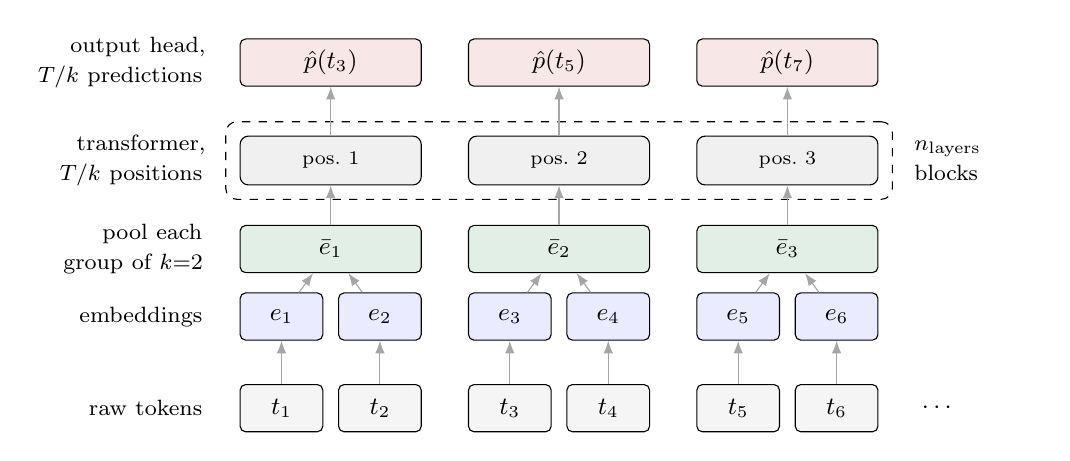
\begin{tikzpicture}[
  font=\small,
  tok/.style={draw, rounded corners=2pt, minimum width=1.05cm,
              minimum height=0.6cm, fill=black!4},
  emb/.style={tok, fill=blue!8},
  pool/.style={tok, minimum width=2.3cm, fill=okgreen!14},
  blk/.style={draw, rounded corners=3pt, minimum width=2.3cm,
              minimum height=0.62cm, fill=black!6},
  pred/.style={tok, minimum width=2.3cm, fill=warnred!12},
  ar/.style={-{Latex[length=1.6mm]}, gray!70},
  node distance=0.42cm and 0.3cm,
]
% raw tokens
\foreach \i/\x in {1/0, 2/1.25, 3/2.9, 4/4.15} {
  \node[tok] (t\i) at (\x, 0) {$t_{\i}$};
}
\node[tok] (t5) at (5.8,0) {$t_5$};
\node[tok] (t6) at (7.05,0) {$t_6$};
\node at (8.35,0) {$\cdots$};
\node[left=0.35cm of t1, align=right, text width=2.1cm]
  {\footnotesize raw tokens};

% embeddings
\foreach \i in {1,...,6} {
  \node[emb, above=0.55cm of t\i] (e\i) {$e_{\i}$};
  \draw[ar] (t\i) -- (e\i);
}
\node[left=0.35cm of e1, align=right, text width=2.1cm]
  {\footnotesize embeddings};

% pooling
\node[pool, above=0.55cm of $(e1)!0.5!(e2)$] (p1) {$\bar e_1$};
\node[pool, above=0.55cm of $(e3)!0.5!(e4)$] (p2) {$\bar e_2$};
\node[pool, above=0.55cm of $(e5)!0.5!(e6)$] (p3) {$\bar e_3$};
\foreach \a/\b in {e1/p1, e2/p1, e3/p2, e4/p2, e5/p3, e6/p3} {
  \draw[ar] (\a) -- (\b);
}
\node[left=0.35cm of p1, align=right, text width=2.1cm]
  {\footnotesize pool each\\group of $k{=}2$};

% transformer
\node[blk, above=0.5cm of p1] (b1) {\scriptsize pos.\ 1};
\node[blk, above=0.5cm of p2] (b2) {\scriptsize pos.\ 2};
\node[blk, above=0.5cm of p3] (b3) {\scriptsize pos.\ 3};
\foreach \a/\b in {p1/b1, p2/b2, p3/b3} {\draw[ar] (\a) -- (\b);}
\begin{scope}[on background layer]
  \node[draw, dashed, rounded corners=4pt, inner sep=5pt,
        fit=(b1)(b3)] (tf) {};
\end{scope}
\node[right=0.15cm of tf, align=left, text width=1.5cm]
  {\footnotesize $n_{\mathrm{layers}}$\\blocks};
\node[left=0.35cm of b1, align=right, text width=2.1cm]
  {\footnotesize transformer,\\$T/k$ positions};

% head
\node[pred, above=0.62cm of b1] (o1) {$\hat p(t_3)$};
\node[pred, above=0.62cm of b2] (o2) {$\hat p(t_5)$};
\node[pred, above=0.62cm of b3] (o3) {$\hat p(t_7)$};
\foreach \a/\b in {b1/o1, b2/o2, b3/o3} {\draw[ar] (\a) -- (\b);}
\node[left=0.35cm of o1, align=right, text width=2.1cm]
  {\footnotesize output head,\\$T/k$ predictions};
\end{tikzpicture}
\caption{Token averaging at $k{=}2$. Raw tokens are embedded as usual, then
every $k$ consecutive embeddings are replaced by one pooled vector before the
first transformer block. The transformer and the output head therefore run on
$T/k$ positions instead of $T$, and each position predicts the first raw token
of the next group. The pooling step is the only change to the architecture;
mean pooling adds no parameters. Rotary position embeddings act on the
compressed positions $1, \dots, T/k$, not on the raw ones.}
\label{fig:arch}
\end{figure}

One point about position is worth noting. Rotary position embeddings are
applied inside the transformer to the \emph{compressed} positions
$1, \dots, n$, so neighbouring transformer positions are always $k$ raw
tokens apart. The compressed sequence therefore looks positionally the same
no matter where the group boundaries fall in the raw text, which matters for
the offset analysis in Section~\ref{sec:offset-ensemble}.

\subsection{Training objective}
\label{sec:method-objective}

We index groups and positions from 1. Group $j$ covers the raw tokens
$t_{(j-1)k+1}, \dots, t_{jk}$, and sits at compressed position $j$ of the
transformer. At that position the model predicts the \emph{first token of the
next group}, which is $t_{jk+1}$: it has seen the first $jk$ raw tokens in
compressed form, and must name the token that comes next. The table below
shows the $k{=}2$ case on eight raw tokens, where $e_i$ is the embedding of
raw token $t_i$.

\begin{center}
\begin{tabular}{lcccccccc}
\toprule
raw tokens & $t_1$ & $t_2$ & $t_3$ & $t_4$ & $t_5$ & $t_6$ & $t_7$ & $t_8$ \\
\midrule
transformer input & \multicolumn{2}{c}{$\bar e_1 = \tfrac{e_1+e_2}{2}$}
               & \multicolumn{2}{c}{$\bar e_2 = \tfrac{e_3+e_4}{2}$}
               & \multicolumn{2}{c}{$\bar e_3 = \tfrac{e_5+e_6}{2}$}
               & \multicolumn{2}{c}{$\bar e_4 = \tfrac{e_7+e_8}{2}$} \\
\midrule
compressed position & \multicolumn{2}{c}{1} & \multicolumn{2}{c}{2}
       & \multicolumn{2}{c}{3} & \multicolumn{2}{c}{4} \\
\midrule
target & \multicolumn{2}{c}{$t_3$}
       & \multicolumn{2}{c}{$t_5$}
       & \multicolumn{2}{c}{$t_7$}
       & \multicolumn{2}{c}{$t_9$} \\
\bottomrule
\end{tabular}
\end{center}

The target at the last compressed position is $t_9$, the first token of the
next group, which lies outside the eight tokens shown. In a real batch $t_9$
is simply the next token of the packed stream and the prediction is scored as
usual; only at the very end of a sequence is there no target, in which case
that one position is dropped.

The loss is ordinary cross-entropy, averaged over all predicted positions.
Two properties of this objective drive much of the paper. First, the model
predicts only the tokens $t_{k+1}, t_{2k+1}, t_{3k+1}, \dots$, one per group.
It never assigns a probability to any other token, which is the root of the
evaluation problem in Section~\ref{sec:offset-ensemble}. Second, each
prediction is made from a lossy view of the past: the most recent group
reaches the model only through its mean, so the order of the tokens inside
that group is lost. Section~\ref{sec:results-pooling} measures what that
costs, and whether other pooling functions recover it.

\subsection{Random-offset training}
\label{sec:method-random-offset}

If the groups always started at the beginning of the sequence, the model
would only ever be asked to predict the raw positions $k{+}1, 2k{+}1,
3k{+}1, \dots$, and would never be asked about any of the others. We remove
that asymmetry directly. At each training step we draw an offset $o \sim
\mathrm{Uniform}\{0, \dots, k{-}1\}$, drop the first $o$ tokens of the batch,
and then group as usual. The groups now cover $(o{+}1 \dots o{+}k)$,
$(o{+}k{+}1 \dots o{+}2k)$, and so on, and the predicted positions become
$o{+}k{+}1, o{+}2k{+}1, \dots$. In other words, the whole pattern of
predictions slides along the text by $o$ tokens. Since $o$ takes each of its
$k$ values about equally often, every token position ends up being predicted
in roughly the same number of steps.

Sequence packing already randomizes where the group boundaries fall
\emph{relative to the underlying documents} (Section~\ref{sec:offset-ensemble});
random offsets additionally make the training signal uniform across
positions. At evaluation the offset is fixed to 0, or swept, as in the
offset-ensemble metric. The only cost is the $o \le k{-}1$ tokens we drop:
they shorten each sequence by less than one group, so the batch loses at most
one prediction per sequence. Nothing else about training changes.

\subsection{Two ways to spend the saving: more data or more context}
\label{sec:configs}

The compute that averaging frees up can be spent on more data or on longer
raw context. We use the first as the paper's method and the second as an
ablation that shows where the first one's gains come from. Throughout,
\texttt{seq\_len} is the number of \emph{raw} tokens per training sequence,
and $\Ltr = \texttt{seq\_len}/k$ is the number of positions the transformer
actually processes.

\begin{description}
  \item[More data (the paper's main setting).] The raw \texttt{seq\_len}
        stays at the baseline's 1024. The transformer length falls to
        $\Ltr = 1024/k$, so each raw token costs about $1/k$ of baseline, and
        the model trains on $k\times$ the raw tokens for the same total
        compute. Every prediction still sees 1024 raw tokens of context; only
        the way that context is represented changes.
  \item[More context (ablation).] Raise \texttt{seq\_len} to $k \times 1024$,
        so that $\Ltr = 1024$ matches the baseline's transformer length. Each
        sequence now packs $k\times$ the raw context into the same amount of
        transformer computation. The cost per raw token is again $1/k$ of
        baseline, so this setting also reaches equal total compute at
        $k\times$ the tokens.
\end{description}

The two settings use identical models, data, and optimization; they differ
only in what the freed compute buys. A third arm tells us whether any effect
of the extra context is specific to averaging: a standard $k{=}1$ model whose
attention window is genuinely widened to 2048 tokens (\texttt{seq\_len} $=
\Ltr = 2048$). This model gets the same 2048 tokens of context the ordinary
way, and it pays for them: doubling the window doubles the attention term in
the cost model of Section~\ref{sec:flops}, so this arm is the more expensive
of the two routes to 2048 tokens of context. Section~\ref{sec:flops} gives the
exact figure at our 50M width.

\subsection{FLOPs accounting}
\label{sec:flops}

We compute all FLOPs from first principles. For a transformer with hidden
size $d$, $n_{\mathrm{layers}}$ layers, and transformer sequence length
$\Ltr$, our architecture (attention with $Q,K,V$ and output projections;
SwiGLU FFN with expansion factor 2.5) costs $23d^2 + 4\Ltr d$
multiply--accumulate FLOPs forward per layer per position: $8d^2$ for the four
attention projections, $15d^2$ for the SwiGLU FFN, and $4\Ltr d$ for the
attention scores and the value aggregation
(Appendix~\ref{app:flops} derives these). Each position also produces one
next-token prediction through the dense vocabulary projection, at $2dV$ FLOPs
forward for the padded vocabulary size $V = 50{,}304$. Multiplying by the
usual $3\times$ for forward plus backward, a run that consumes $D$ raw tokens
at raw sequence length \texttt{seq\_len} costs
\begin{equation}
\mathrm{FLOPs}(D)
= \frac{3D}{k}
  \Bigl[\, n_{\mathrm{layers}} \left( 23 d^2 + 4 \Ltr d \right)
        \;+\; 2 d V \,\Bigr],
\qquad \Ltr = \texttt{seq\_len}/k .
\label{eq:flops}
\end{equation}
We include the output projection because at these scales it is a large part
of the bill and not a rounding error. Evaluating Eq.~\eqref{eq:flops} at each
of our four configurations, the $2dV$ term accounts for $44.2\%$, $27.8\%$,
$18.5\%$ and $12.0\%$ of the baseline's total training FLOPs at 50M, 125M,
250M and 500M respectively. The reason it is so large at the small end is
that the vocabulary dwarfs the width: $V \approx 98\,d$ at $d = 512$, and even
at $d = 1280$ it is still $V \approx 39\,d$. Widening the model shrinks this
share, because the body's $23d^2$ term grows quadratically in $d$ while the
head's $2dV$ term grows only linearly. One consequence is worth flagging: the
same 2048-token full-attention arm above costs $1.14\times$ the baseline per
raw token at $\dmodel{=}512$ under this equation.

Equation~\eqref{eq:flops} makes the arithmetic of the more-data setting
clear. Two comparisons are easy to blur, so we separate them.

\emph{At a fixed number of raw tokens} $D$, averaging processes $D/k$
positions instead of $D$. The two terms that are linear in the position
count, the $23d^2$ per layer and the $2dV$ head, therefore fall by a factor
$k$ per raw token. The attention term falls by $k^2$: one factor $k$ from
having fewer positions, and another because each of those positions attends
over a sequence $k$ times shorter.

\emph{At equal total compute}, the averaged run converts that saving into
$kD$ raw tokens. The two linear terms then return \emph{exactly} to the
baseline's totals, because the averaged arm now runs the same number of
transformer positions and makes the same number of predictions as the
baseline. All that is left of its advantage is the attention term, which is
still lower because each position attends over $\Ltr/k$ positions rather than
$\Ltr$. That attention term is the whole of the free saving under our
accounting, and it is small. At equal compute the averaged arm's final cost is
$0.928\times$ the baseline at 50M, $0.932\times$ at 125M, $0.940\times$ at
250M and $0.946\times$ at 500M, and the ratio rises towards $1$ with scale
because attention is a smaller share of the per-position cost as $d$ grows at
fixed $\Ltr$. So what token averaging buys is \emph{data throughput}.
$k\times$ more raw data flows through the same number of positions, with a
modest attention saving on top. What that throughput is worth in loss is the
empirical question.

These particular ratios are a property of this architecture, not of token
averaging in general. The residual saving at equal compute is entirely the
attention term, so anything that changes attention's share of the per-position
cost changes the number. A model with a wider FFN, grouped-query or
multi-query attention, a smaller vocabulary, or a longer $\Ltr$ would land
somewhere else, and a linear-attention or state-space backbone, where the cost
does not grow with sequence length, would leave no residual saving at all. The
$k\times$ data throughput, by contrast, follows from processing $1/k$ as many
positions and holds for any backbone. Readers porting these numbers to another
architecture should recompute the ratio from their own cost model rather than
reuse ours.

\begin{figure}[t]
  \centering
  \begin{subfigure}[b]{0.32\textwidth}
    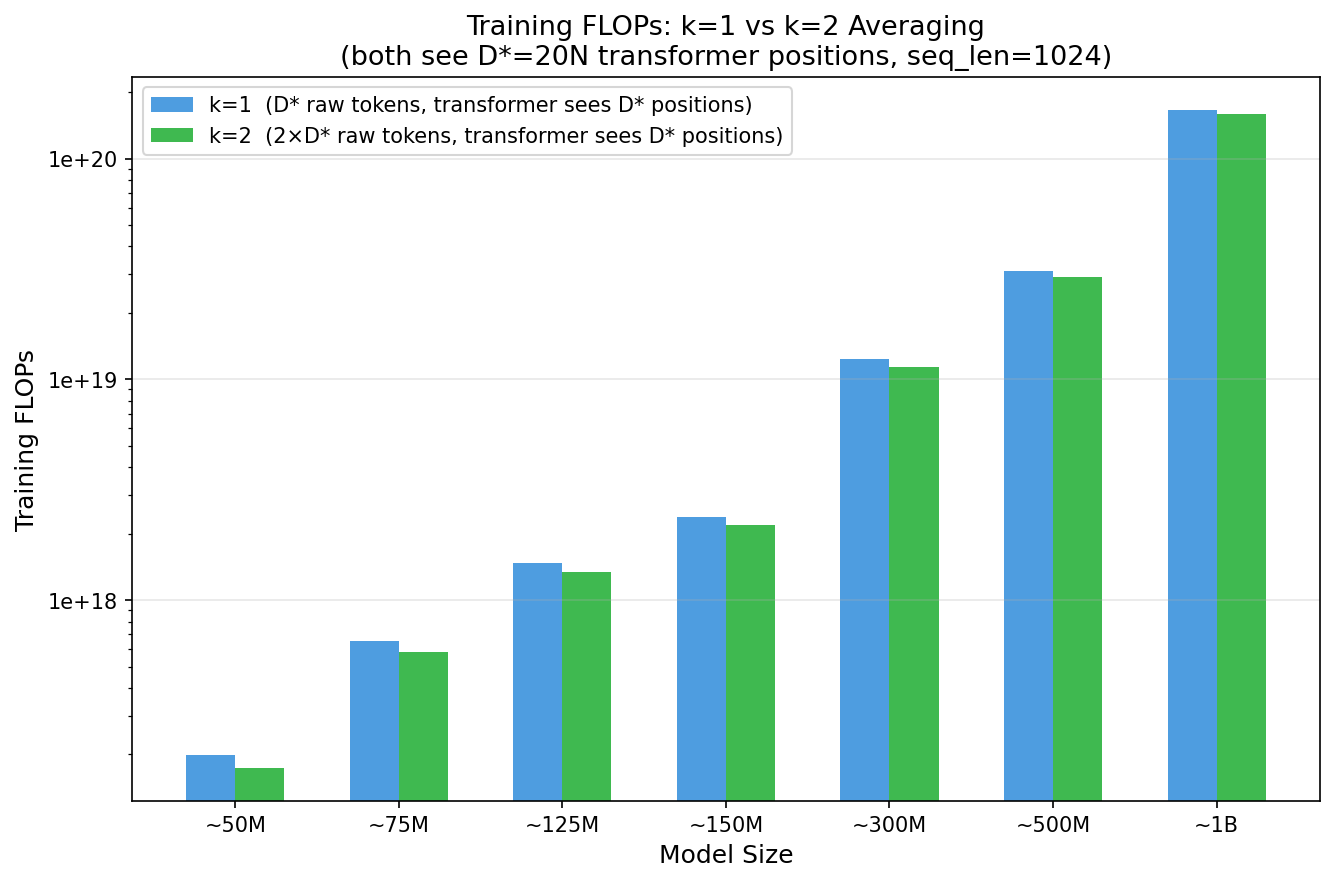
\includegraphics[width=\textwidth]{flops_scaling_absolute.png}
  \end{subfigure}\hfill
  \begin{subfigure}[b]{0.32\textwidth}
    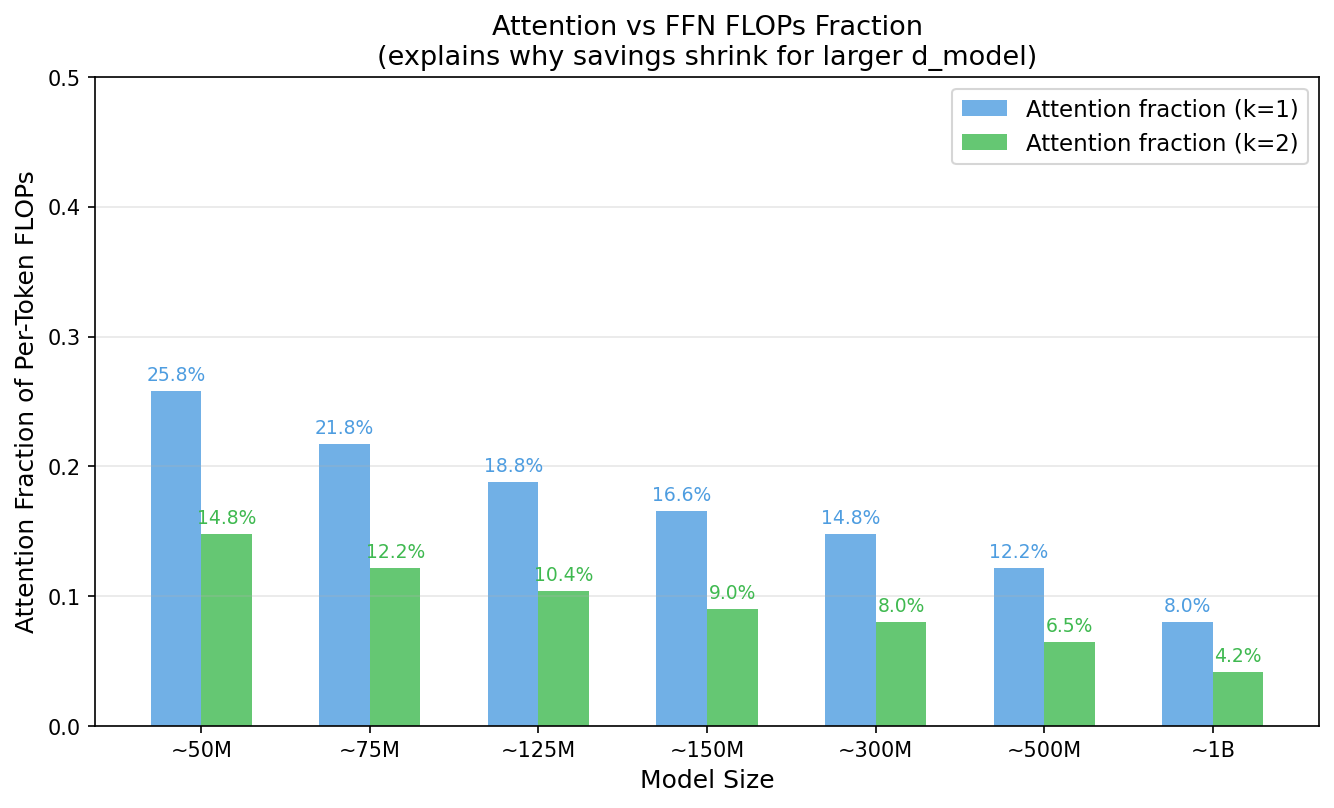
\includegraphics[width=\textwidth]{flops_scaling_attention_fraction.png}
  \end{subfigure}\hfill
  \begin{subfigure}[b]{0.32\textwidth}
    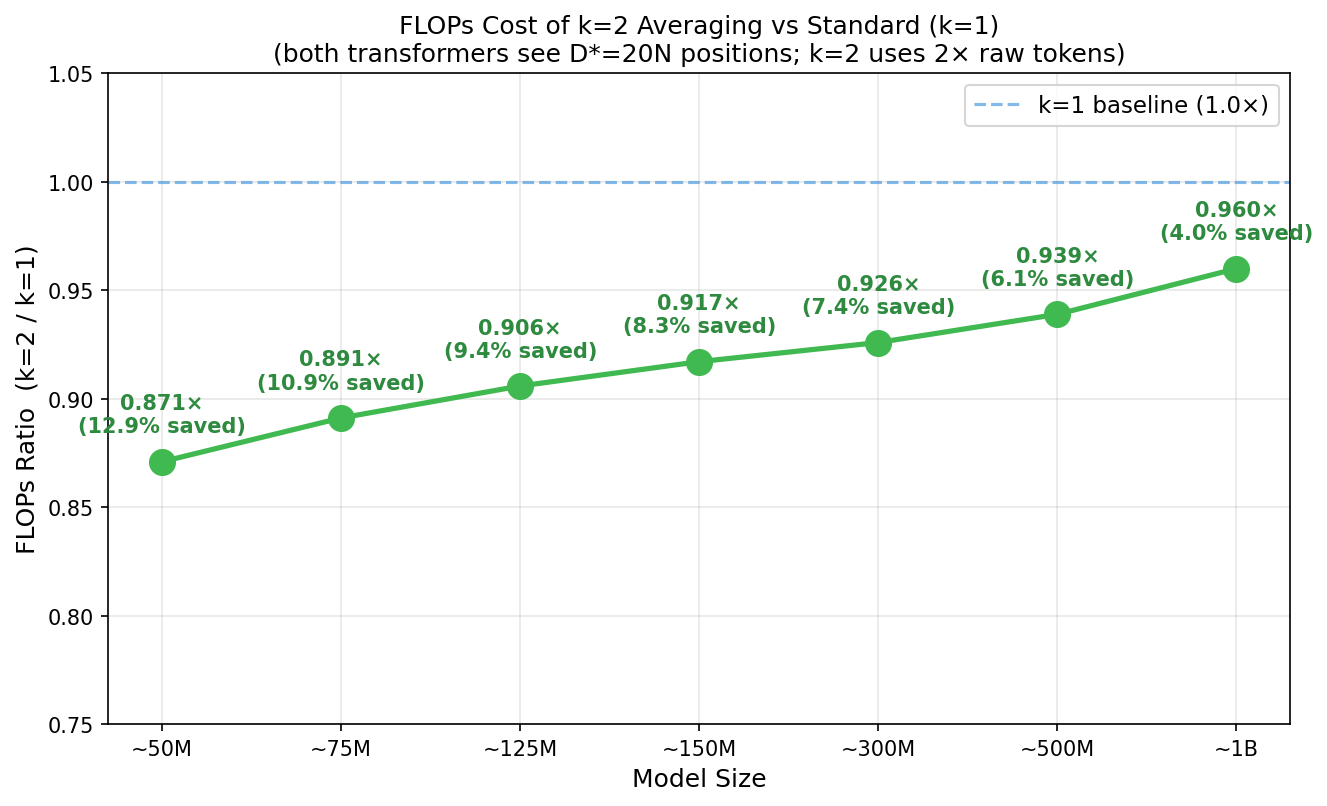
\includegraphics[width=\textwidth]{flops_scaling_ratio.png}
  \end{subfigure}
  \caption{Structure of the transformer-body FLOPs across model widths
  (the output projection of Eq.~\eqref{eq:flops} is excluded from these three
  panels, which are about the body's internal composition). \textbf{Left:}
  absolute body FLOPs per raw token. \textbf{Middle:} the attention share of
  per-position body compute shrinks with $\dmodel$. \textbf{Right:} the
  per-token body FLOPs ratio of $k{=}2$ averaging to baseline at $2\times$ the
  data, across widths. The $k\times$ data throughput does not depend on width;
  the attention saving is what remains at equal compute, and it is largest at
  small widths, which is why the final ratio in Table~\ref{tab:main} rises
  towards $1$ with scale.}
  \label{fig:flops-scaling}
\end{figure}

\subsection{The evaluation problem and the offset-ensemble fix}
\label{sec:offset-ensemble}

\paragraph{The problem.}
The number that defines a language model is the full-sequence log-likelihood
$\sum_i \log p(t_i \mid t_{<i})$. The $k{=}1$ baseline's eval loss is the mean
of all $T{-}1$ of those terms per sequence. A $k$-averaged model's eval loss,
as trained, is the mean over only the ${\sim}T/k$ positions it predicts,
because it has no probability to report for the rest. The two numbers are
therefore averages over \emph{different sets of terms}, and more evaluation
data does not fix that: evaluating the averaged model on $k\times$ as many
batches matches the number of predictions, not the task. The same limitation
affects generation: a model that predicts one token per group cannot decode one
token at a time as trained.

\paragraph{The fix.}
At evaluation time, run the model $k$ times over each sequence, shifting the
group boundaries by $o = 0, 1, \dots, k{-}1$ raw tokens. At offset $o$ the
groups cover tokens $(o{+}1 \dots o{+}k)$, $(o{+}k{+}1 \dots o{+}2k)$, and so
on, and the model's targets are the raw positions $o + jk + 1$ for
$j = 1, 2, \dots$, that is $t_{o+k+1}, t_{o+2k+1}, \dots$ Across the $k$
offsets these target sets never overlap, and together they cover every
position past the first group, each predicted exactly once from its full
compressed prefix. The table below shows the two passes at $k{=}2$ on eight
raw tokens. Each column is scored exactly once across the two passes, so the
union of the two target sets is every position from $t_3$ onwards.

\begin{center}
\begin{tabular}{lcccccccc}
\toprule
raw position & $t_1$ & $t_2$ & $t_3$ & $t_4$ & $t_5$ & $t_6$ & $t_7$ & $t_8$ \\
\midrule
offset $o{=}0$: groups
  & \multicolumn{2}{c}{$[t_1 t_2]$} & \multicolumn{2}{c}{$[t_3 t_4]$}
  & \multicolumn{2}{c}{$[t_5 t_6]$} & \multicolumn{2}{c}{$[t_7 t_8]$} \\
\phantom{offset $o{=}0$: }targets
  & -- & -- & \checkmark & -- & \checkmark & -- & \checkmark & -- \\
\midrule
offset $o{=}1$: groups
  & drop & \multicolumn{2}{c}{$[t_2 t_3]$} & \multicolumn{2}{c}{$[t_4 t_5]$}
  & \multicolumn{2}{c}{$[t_6 t_7]$} & $\cdots$ \\
\phantom{offset $o{=}1$: }targets
  & -- & -- & -- & \checkmark & -- & \checkmark & -- & \checkmark \\
\bottomrule
\end{tabular}
\end{center}

The result is a genuine full-sequence NLL over all scored
positions, directly comparable to the baseline's on the same positions. It
costs $k$ forward passes over sequences of length $\Ltr = T/k$, so about
\emph{one} baseline forward pass in total. We also score the baseline on
exactly this set of positions, so that the two numbers cover the same
predictions and not merely the same number of them. The same idea gives a
decoding scheme: while generating, rotate the offset so that a group boundary
always ends at the current position. This needs $k$ KV caches, one per offset,
but each is $1/k$ the length, so the total cost is about that of one ordinary
decoder (Appendix~\ref{app:offset}).

\paragraph{Why every offset works about as well.}
Random-offset training (Section~\ref{sec:method-random-offset}) makes the
model see all $k$ offsets while training. Two further facts mean it would
largely handle them anyway. First, training sequences are cut from a
continuous token stream into fixed-length chunks, and those cuts fall at
arbitrary points inside documents, so the group boundaries are already
uniformly random \emph{relative to the text} whichever offset we use. Second,
RoPE acts on compressed positions (Section~\ref{sec:method-averaging}), so the
positional geometry the transformer sees is the same at every offset. The
measured per-offset losses bear this out: they are essentially equal
(Section~\ref{sec:results-fullpos}).

\subsection{Pooling functions}
\label{sec:method-pooling}

Everything the transformer sees passes through the pooling function, so we
vary it while holding everything else fixed. Each variant below compresses a
group of embeddings into one vector and leaves the rest of the pipeline
untouched.

\begin{description}
  \item[Mean (default).] Equal weights $1/k$. No parameters.
  \item[Fixed recency weights.] $\bar e = \sum_i w_i e_i$ with $w_i \propto
        \exp(\alpha i)$, where $\alpha$ is chosen so the last token of a group
        weighs 20 times the first, then $L_1$-normalized. This is a pure
        recency rule with no learned parameters: the token closest to the
        prediction target dominates. (We also implemented linear, Gaussian,
        and triangular profiles; the exponential one is the version we
        trained.)
  \item[Learned from content only.] A single shared linear scorer assigns a
        score $s_i = w^\top e_i + b$ to the $i$-th token of a group, where
        $w \in \mathbb{R}^{\dmodel}$ and $b \in \mathbb{R}$ are shared by all
        slots and all groups. The scores are turned into weights within the
        group by $\alpha = \mathrm{softmax}(s_{1..k})$, and the pooled vector
        is $\bar e = \sum_i \alpha_i e_i$. This adds $\dmodel + 1 = 513$
        parameters, initialized at zero so training starts exactly at mean
        pooling. Note that $b$ is the same for every slot, and softmax is
        unchanged by adding a constant to all its inputs, so $b$ has no effect
        on the weights; it is there only because it comes with the linear
        layer. The scorer sees each embedding on its own, \emph{before} the
        network has any positional information, so it can react to what a
        token is but not to where in the group it sits. That turns out to
        matter (Section~\ref{sec:results-pooling}).
  \item[Learned from content and position.] The same scorer plus one learned
        bias per slot of the group: $s_i = w^\top e_i + b + p_i$, with
        $p \in \mathbb{R}^k$ trained jointly, for $\dmodel + 1 + k$
        parameters. Each $p_i$ is a single number, but unlike $b$ there is a
        \emph{different} one for each slot $i$, so the $p_i$ do not cancel in
        the softmax. Only their differences matter, which leaves $k{-}1$
        effective degrees of freedom. What $p$ learns is therefore a fixed
        profile over slots, applied to every group in the corpus, and in
        practice it puts more weight on the later slots. In that sense it is a
        learned version of the fixed recency rule above rather than anything
        richer: the score is the sum of a content term and a position term, so
        the module cannot represent an interaction between the two, such as
        ``this token matters because of what it is \emph{and} where it sits.''
        We call it position-aware for that reason and no stronger one. We
        initialize $p$ uniform at $k{=}2$ and at the exponential recency
        profile at $k{=}4$, which is the best fixed rule we found at each
        compression ratio, so the model starts from the strongest prior we
        know of and can then adapt both terms.
  \item[Overlapping groups.] Average groups of $w{=}4$ tokens with stride
        $s{=}2$. This gives the same $2\times$ compression as $k{=}2$, but
        neighbouring groups share tokens, so no token sits on a hard boundary.
        Targets are the first token past each group.
  \item[Word-aligned groups.] Groups of variable size (at least $k$ tokens,
        force-closed at $2k$) that end only at word boundaries, detected from
        the tokenizer's whitespace-prefix convention, so no group straddles two
        words. Because a group only closes at a word boundary, it often runs
        past $k$ tokens, so the realized compression is above the nominal
        $k$. We measured it rather than assumed it: on a tokenized sample of
        English text the mean group size is $2.125$ at $k{=}2$, a realized
        compression of ${\sim}2.1\times$. The predicted positions are also
        word starts rather than arbitrary positions. Both facts affect
        comparability, and we handle them in Appendix~\ref{app:word}.
\end{description}

% =====================================================================
\section{Experimental Setup}
% =====================================================================
\label{sec:setup}

\paragraph{Architecture.}
All models are GPT-NeoX-style decoder-only transformers built from the OLM
implementation: pre-norm blocks, rotary position embeddings, SwiGLU FFN with
expansion factor 2.5, and a padded vocabulary of 50{,}304 (tokenizer
vocabulary 50{,}257). Apart from the pooling step of
Figure~\ref{fig:arch}, which sits between the embedding table and the first
block, the averaged models are architecturally identical to the baselines.
Table~\ref{tab:models} lists the four scales. Input and output embeddings are
tied at all scales.

\begin{table}[h]
\centering
\caption{Model configurations. ``Raw tokens'' are the training budgets for
the $k{=}1$ / $k{=}2$ arms, set so both arms end at approximately equal
total training FLOPs (Eq.~\ref{eq:flops}); the $k{=}1$ budgets follow the
Chinchilla $D^\ast \approx 20N$ heuristic. All main runs use raw
\texttt{seq\_len} = 1024, the more-data setting.}
\label{tab:models}
\vspace{0.4em}
\begin{tabular}{lcccccc}
\toprule
Scale & Params & $\dmodel$ & Heads & Layers & LR & Raw tokens ($k{=}1$ / $k{=}2$) \\
\midrule
50M  & 50.9M  & 512  & 8  & 8  & $2.0\times10^{-4}$ & 1B / 2B \\
125M & 123.5M & 768  & 12 & 12 & $1.6\times10^{-4}$ & 2.5B / 5B \\
250M & 252.8M & 1024 & 16 & 16 & $1.4\times10^{-4}$ & 5B / 10B \\
500M & 479.3M & 1280 & 20 & 22 & $1.2\times10^{-4}$ & 10B / 20B \\
\bottomrule
\end{tabular}
\end{table}

\paragraph{Data and tokenization.}
All models train from scratch on FineWeb, tokenized with the EleutherAI
Pythia-70m (GPT-NeoX) BPE tokenizer. Runs up to and including 250M draw from
\texttt{sample-10BT}. The 500M pair does not fit in that slice, because its
$k{=}2$ arm alone consumes 20B raw tokens, so both 500M arms draw from
\texttt{sample-100BT} instead. We change the slice for both arms of the pair,
so it does not affect the comparison between them.
The token stream is packed into fixed-length sequences without
document-boundary masking. That is standard practice, and it matters for the
context experiments (Section~\ref{sec:results-context}). Evaluation uses a
held-out split of the same distribution, identical across all arms of a
comparison.

\paragraph{Optimization.}
AdamW with a cosine learning-rate schedule: 2{,}000 warmup steps, decay to
$10\%$ of peak over exactly the run's total step count. Peak learning rates
follow Table~\ref{tab:models}. Mixed-precision (bfloat16) training on
NVIDIA GPUs via PyTorch DDP; gradient checkpointing at 250M but not at 500M,
where memory-efficient attention made it unnecessary and it measurably
reduced throughput. Batch sizes and step counts per run are tabulated in
Appendix~\ref{app:runs}.

\paragraph{Budgets and equal-compute design.}
At each scale the $k{=}1$ arm trains on about $20N$ raw tokens and the $k{=}2$
arm on twice that. By Eq.~\eqref{eq:flops} this puts the two endpoints at
about equal training FLOPs: exactly equal in the two linear terms, and in fact
slightly \emph{below} the baseline for the $k{=}2$ arm because its attention
term is smaller ($0.928\times$ at 50M, $0.932\times$ at 125M, $0.940\times$ at
250M, $0.946\times$ at 500M). The ratio rises towards $1$ with scale, because
attention is a smaller fraction of the per-position cost as $\dmodel$ grows at
fixed $\Ltr$.

We read every curve two ways. Vertically, at equal compute, we compare loss.
Horizontally, at equal loss, we compare compute. Both are needed because
late-training loss curves are very flat, so a small vertical gap corresponds
to a large horizontal one.

\paragraph{Metrics.}
Two metrics appear in this paper, and each has a fixed job. \textbf{Native
eval loss} is cross-entropy in nats per predicted token on held-out data, at
whatever positions the model natively predicts (offset 0). It is what training
logs, and we use it for training curves and for comparing runs that share the
same $k$ and grouping scheme. \textbf{Full-position NLL} is the
offset-ensemble metric of Section~\ref{sec:offset-ensemble}. It scores every
position of the identical evaluation sequences, and it is the metric for every
comparison across $k$. We evaluate all final checkpoints under both.
\todo{fill in full-position numbers for the 50M and 250M pairs and the
context arms as runs complete}

% =====================================================================
\section{Results}
% =====================================================================
\label{sec:results}

\subsection{Equal-compute comparison}
\label{sec:results-main}

This subsection covers the four more-data pairs, one per model scale. In each
pair a $k{=}1$ baseline and a $k{=}2$ averaged model are trained to the same
compute budget, the averaged arm on twice the raw tokens. We report their
training curves and their final losses. These are native losses, so each
model is scored on the positions it was trained to predict. The comparison on
the offset-ensemble metric, which scores both models on the same positions
and is the metric behind every conclusion we draw across $k$, follows in
Section~\ref{sec:results-fullpos}.

\begin{figure}[t]
  \centering
  \begin{subfigure}[b]{0.49\textwidth}
    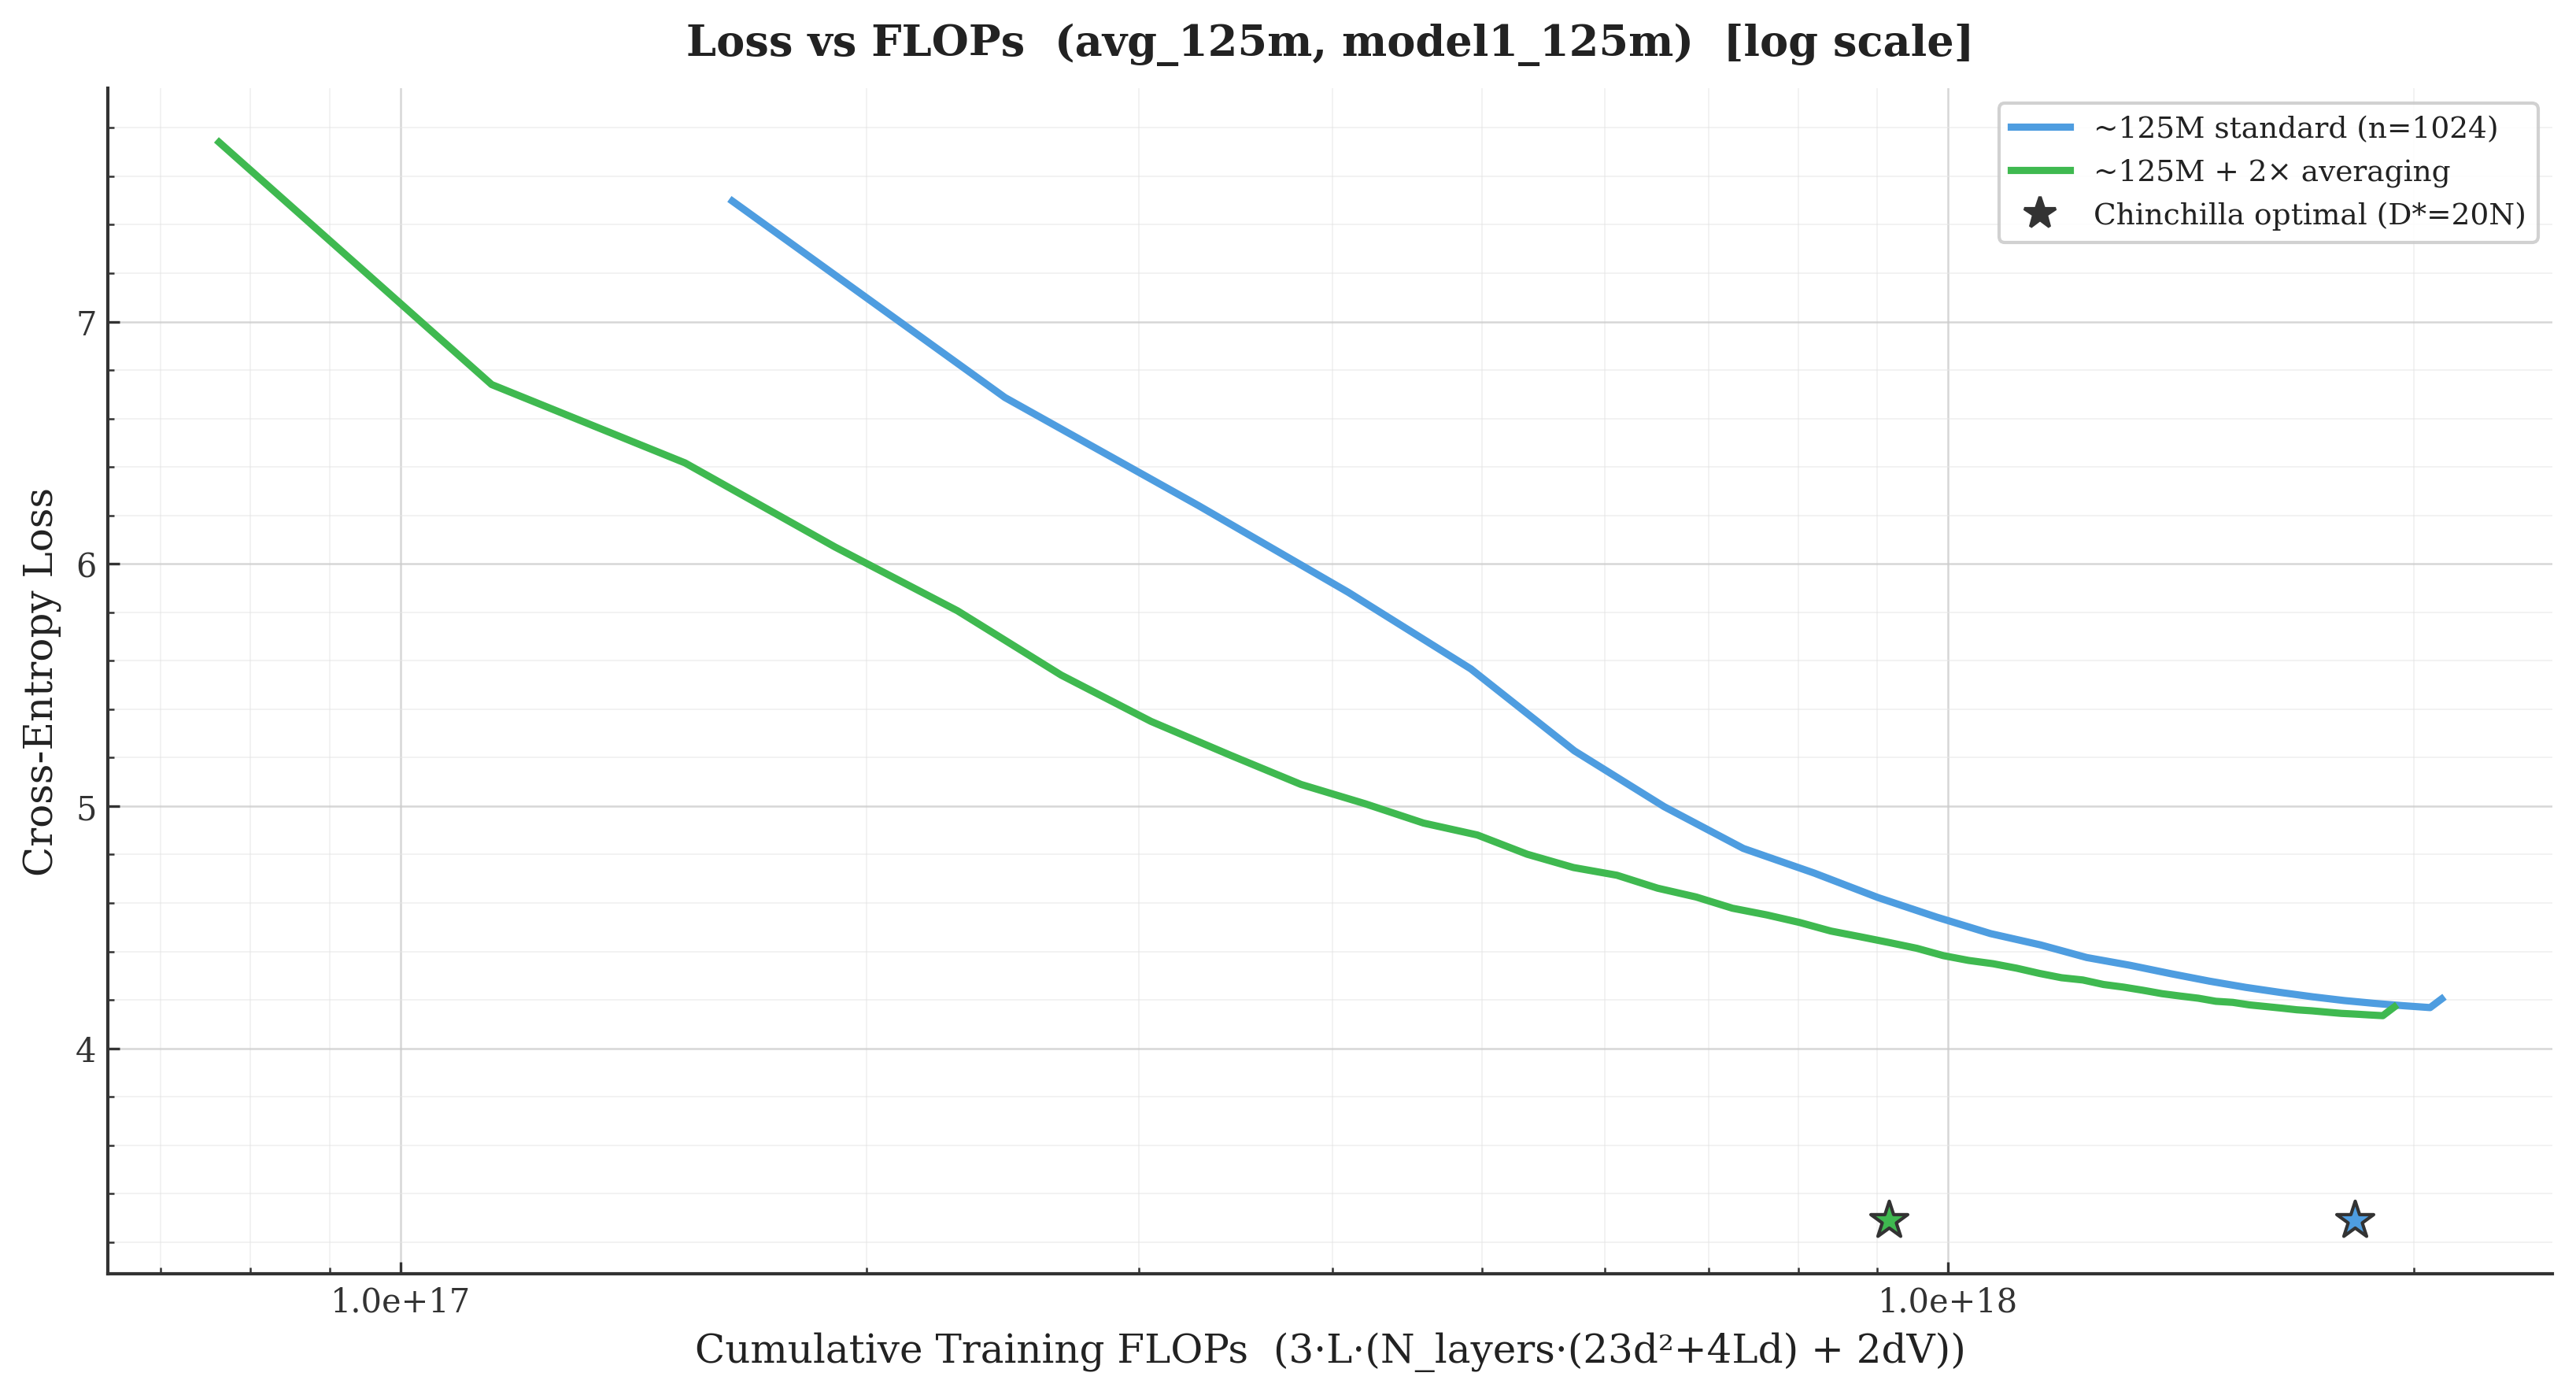
\includegraphics[width=\textwidth]{125m_loss_vs_flops_log.png}
    \caption{Loss vs.\ training FLOPs (log $x$).}
  \end{subfigure}\hfill
  \begin{subfigure}[b]{0.49\textwidth}
    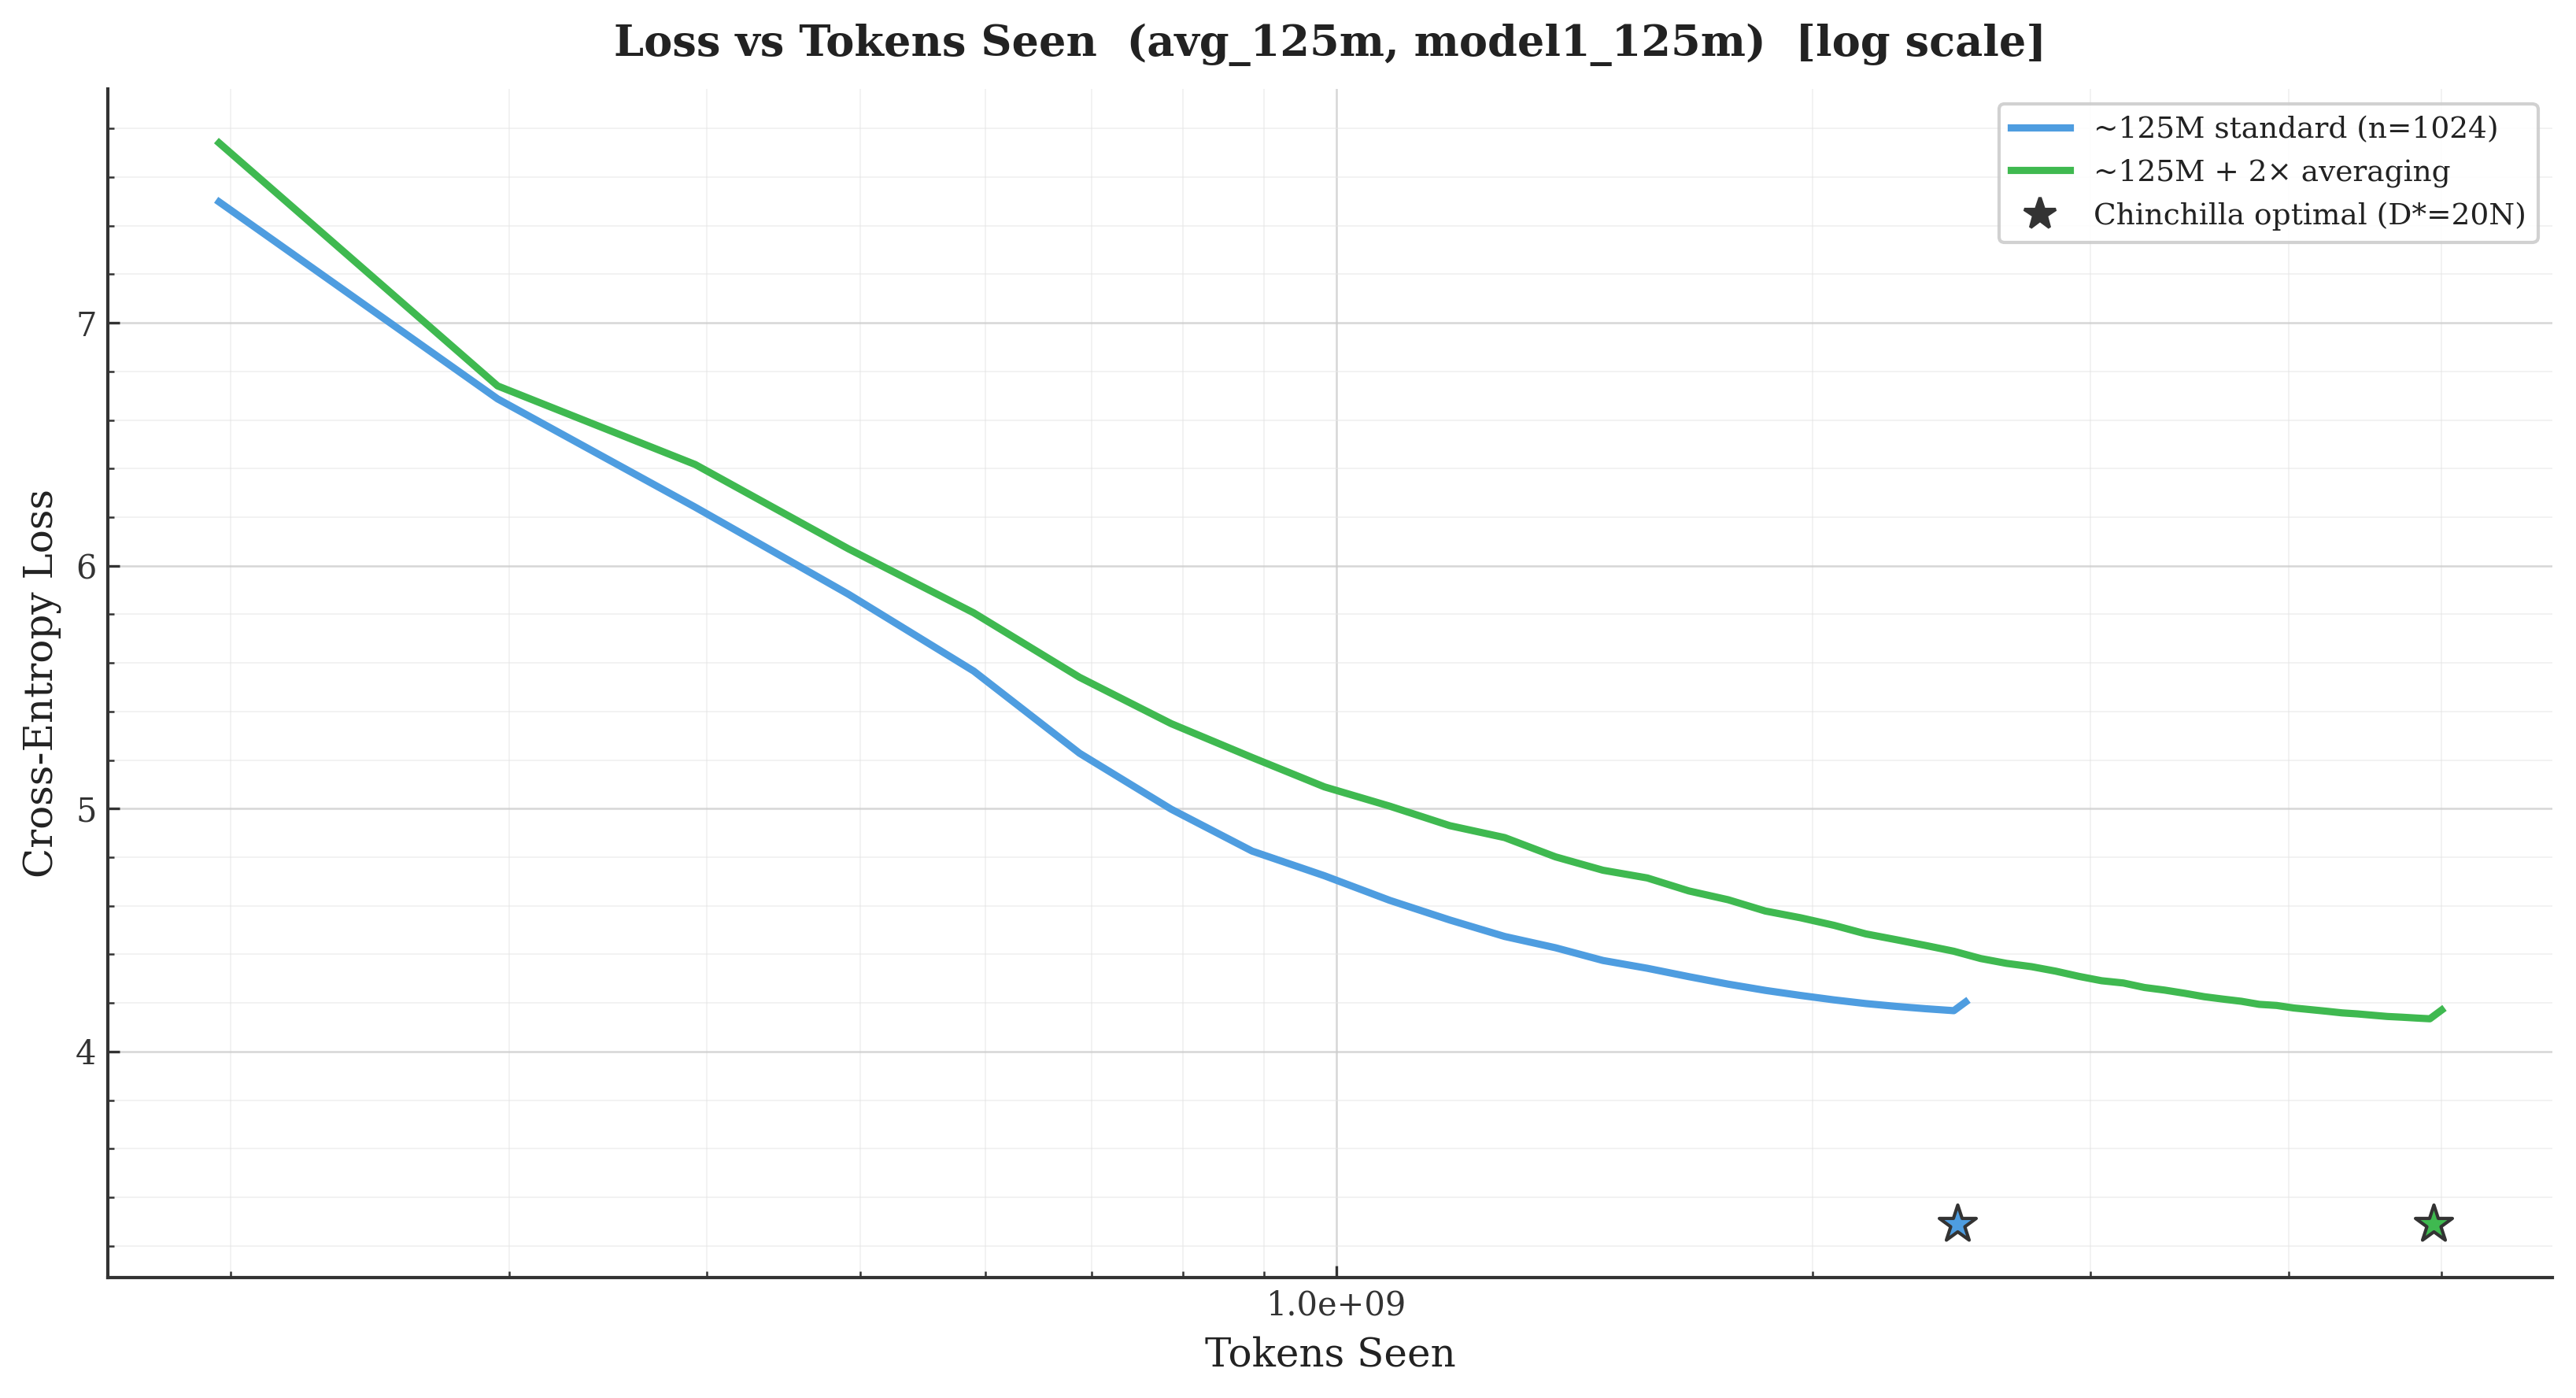
\includegraphics[width=\textwidth]{125m_loss_vs_tokens_log.png}
    \caption{Loss vs.\ raw tokens seen (log $x$).}
  \end{subfigure}
  \caption{125M comparison, native eval losses. On the FLOPs axis (left)
  the $k{=}2$ curve sits below the baseline curve along the whole
  trajectory at equal FLOPs; the endpoint comparison on the full-position
  metric is in Section~\ref{sec:results-fullpos}. On the raw-token axis
  (right) the averaged model learns slightly \emph{less} per token
  (averaging is lossy), but each of its tokens costs roughly half the
  compute. Stars mark Chinchilla-optimal reference points
  ($D^\ast{=}20N$).}
  \label{fig:125m}
\end{figure}

Figure~\ref{fig:125m} shows the 125M pair; Table~\ref{tab:main} summarizes
endpoints at all scales. Three observations.

\begin{table}[h]
\centering
\caption{Main equal-compute comparison (more-data setting, raw
\texttt{seq\_len} 1024). Losses are final native eval CE (nats/token) at each
model's own prediction positions; the comparison across $k$ on the
full-position metric is in Section~\ref{sec:results-fullpos}. Train FLOPs are
computed from tokens seen via Eq.~\eqref{eq:flops} in all rows. The equal-loss
saving is read horizontally off the loss--FLOPs curves
(Appendix~\ref{app:equalloss}). At 500M the two arms end a few thousandths of
a nat apart and in opposite orders on the two metrics, so we quote no
equal-loss saving there.
\todo{add 1B}}
\label{tab:main}
\vspace{0.4em}
\small
\setlength{\tabcolsep}{4.5pt}
\begin{tabular}{llccccc}
\toprule
Scale & Arm & Raw tokens & Train FLOPs & Final eval & vs.\ base & Saving \\
\midrule
50M  & $k{=}1$ & 1.0B & $3.50\times10^{17}$ & 4.437 & -- & \\
50M  & $k{=}2$ & 2.0B & $3.24\times10^{17}$ & \good{4.363} & $0.928\times$ & \good{$1.48\times$} \\
\midrule
125M & $k{=}1$ & 2.5B & $2.08\times10^{18}$ & 4.204 & -- & \\
125M & $k{=}2$ & 5.0B & $1.94\times10^{18}$ & \good{4.171} & $0.932\times$ & \good{$1.43\times$} \\
\midrule
250M & $k{=}1$ & 5.0B & $8.34\times10^{18}$ & 3.414 & -- & \\
250M & $k{=}2$ & 10.0B & $7.84\times10^{18}$ & \good{3.403} & $0.940\times$ & \good{$1.31\times$} \\
\midrule
500M & $k{=}1$ & 10.0B & $3.22\times10^{19}$ & 3.105 & -- & \\
500M & $k{=}2$ & 20.0B & $3.05\times10^{19}$ & 3.107 & $0.946\times$ & n/a \\
\bottomrule
\end{tabular}
\end{table}

First, the averaged model ends below the baseline at 50M, 125M and 250M, and
it spends fewer FLOPs to get there ($0.928\times$ at 50M, $0.932\times$ at
125M, $0.940\times$ at 250M, $0.946\times$ at 500M). The gaps at the end of
training are small: $0.074$ nats at 50M, $0.033$ at 125M and $0.011$ at 250M.
At 500M the two arms end $0.003$ nats apart on this metric, with the baseline
just ahead.

Reading the curves horizontally is more useful than reading them at the end.
At 125M the baseline needs its full $2.08\times10^{18}$ FLOPs to reach loss
4.204, and the averaged model reaches that same loss at
$1.46\times10^{18}$, so the baseline needs \good{$1.43\times$} the compute.
The same reading gives \good{$1.48\times$} at 50M and \good{$1.31\times$} at
250M. We take the target loss from the baseline's last logged evaluation and
find where the averaged run's curve crosses it, interpolating between the two
logged points that bracket the crossing. Appendix~\ref{app:equalloss} gives
the numbers behind each reading and the script that produces them. We quote no
multiplier at 500M, because the two curves finish close enough together that
the crossing point moves a long way between adjacent logged evaluations.

One caveat applies to all of these readings. Native losses for $k{=}1$ and
$k{=}2$ average over different sets of predictions
(Section~\ref{sec:offset-ensemble}), so the two curves are not measuring the
same task. Each curve is good evidence about its own family, but a multiplier
read across two curves is provisional until we repeat the reading on the
offset-ensemble metric. We have that metric at 125M and 500M and it agrees
with the direction of the native result at both
(Section~\ref{sec:results-fullpos}). The 50M and 250M pairs still need
rescoring. The 500M pair is a good illustration of why the native metric
cannot settle a comparison across $k$: the native and offset-ensemble metrics
put the two arms in opposite orders there, and both differences are a few
thousandths of a nat.

Second, the raw-token view (Figure~\ref{fig:125m}b) shows the mechanism
directly. Per raw token the averaged model learns \emph{slightly less} than
the baseline, because compression does lose information. But it processes each
token at roughly half the compute, and the trade nets out positive. Token
averaging does not make the model better per token. It makes tokens cheap
enough that seeing twice as many is worth it.

\begin{figure}[t]
  \centering
  \begin{subfigure}[b]{0.49\textwidth}
    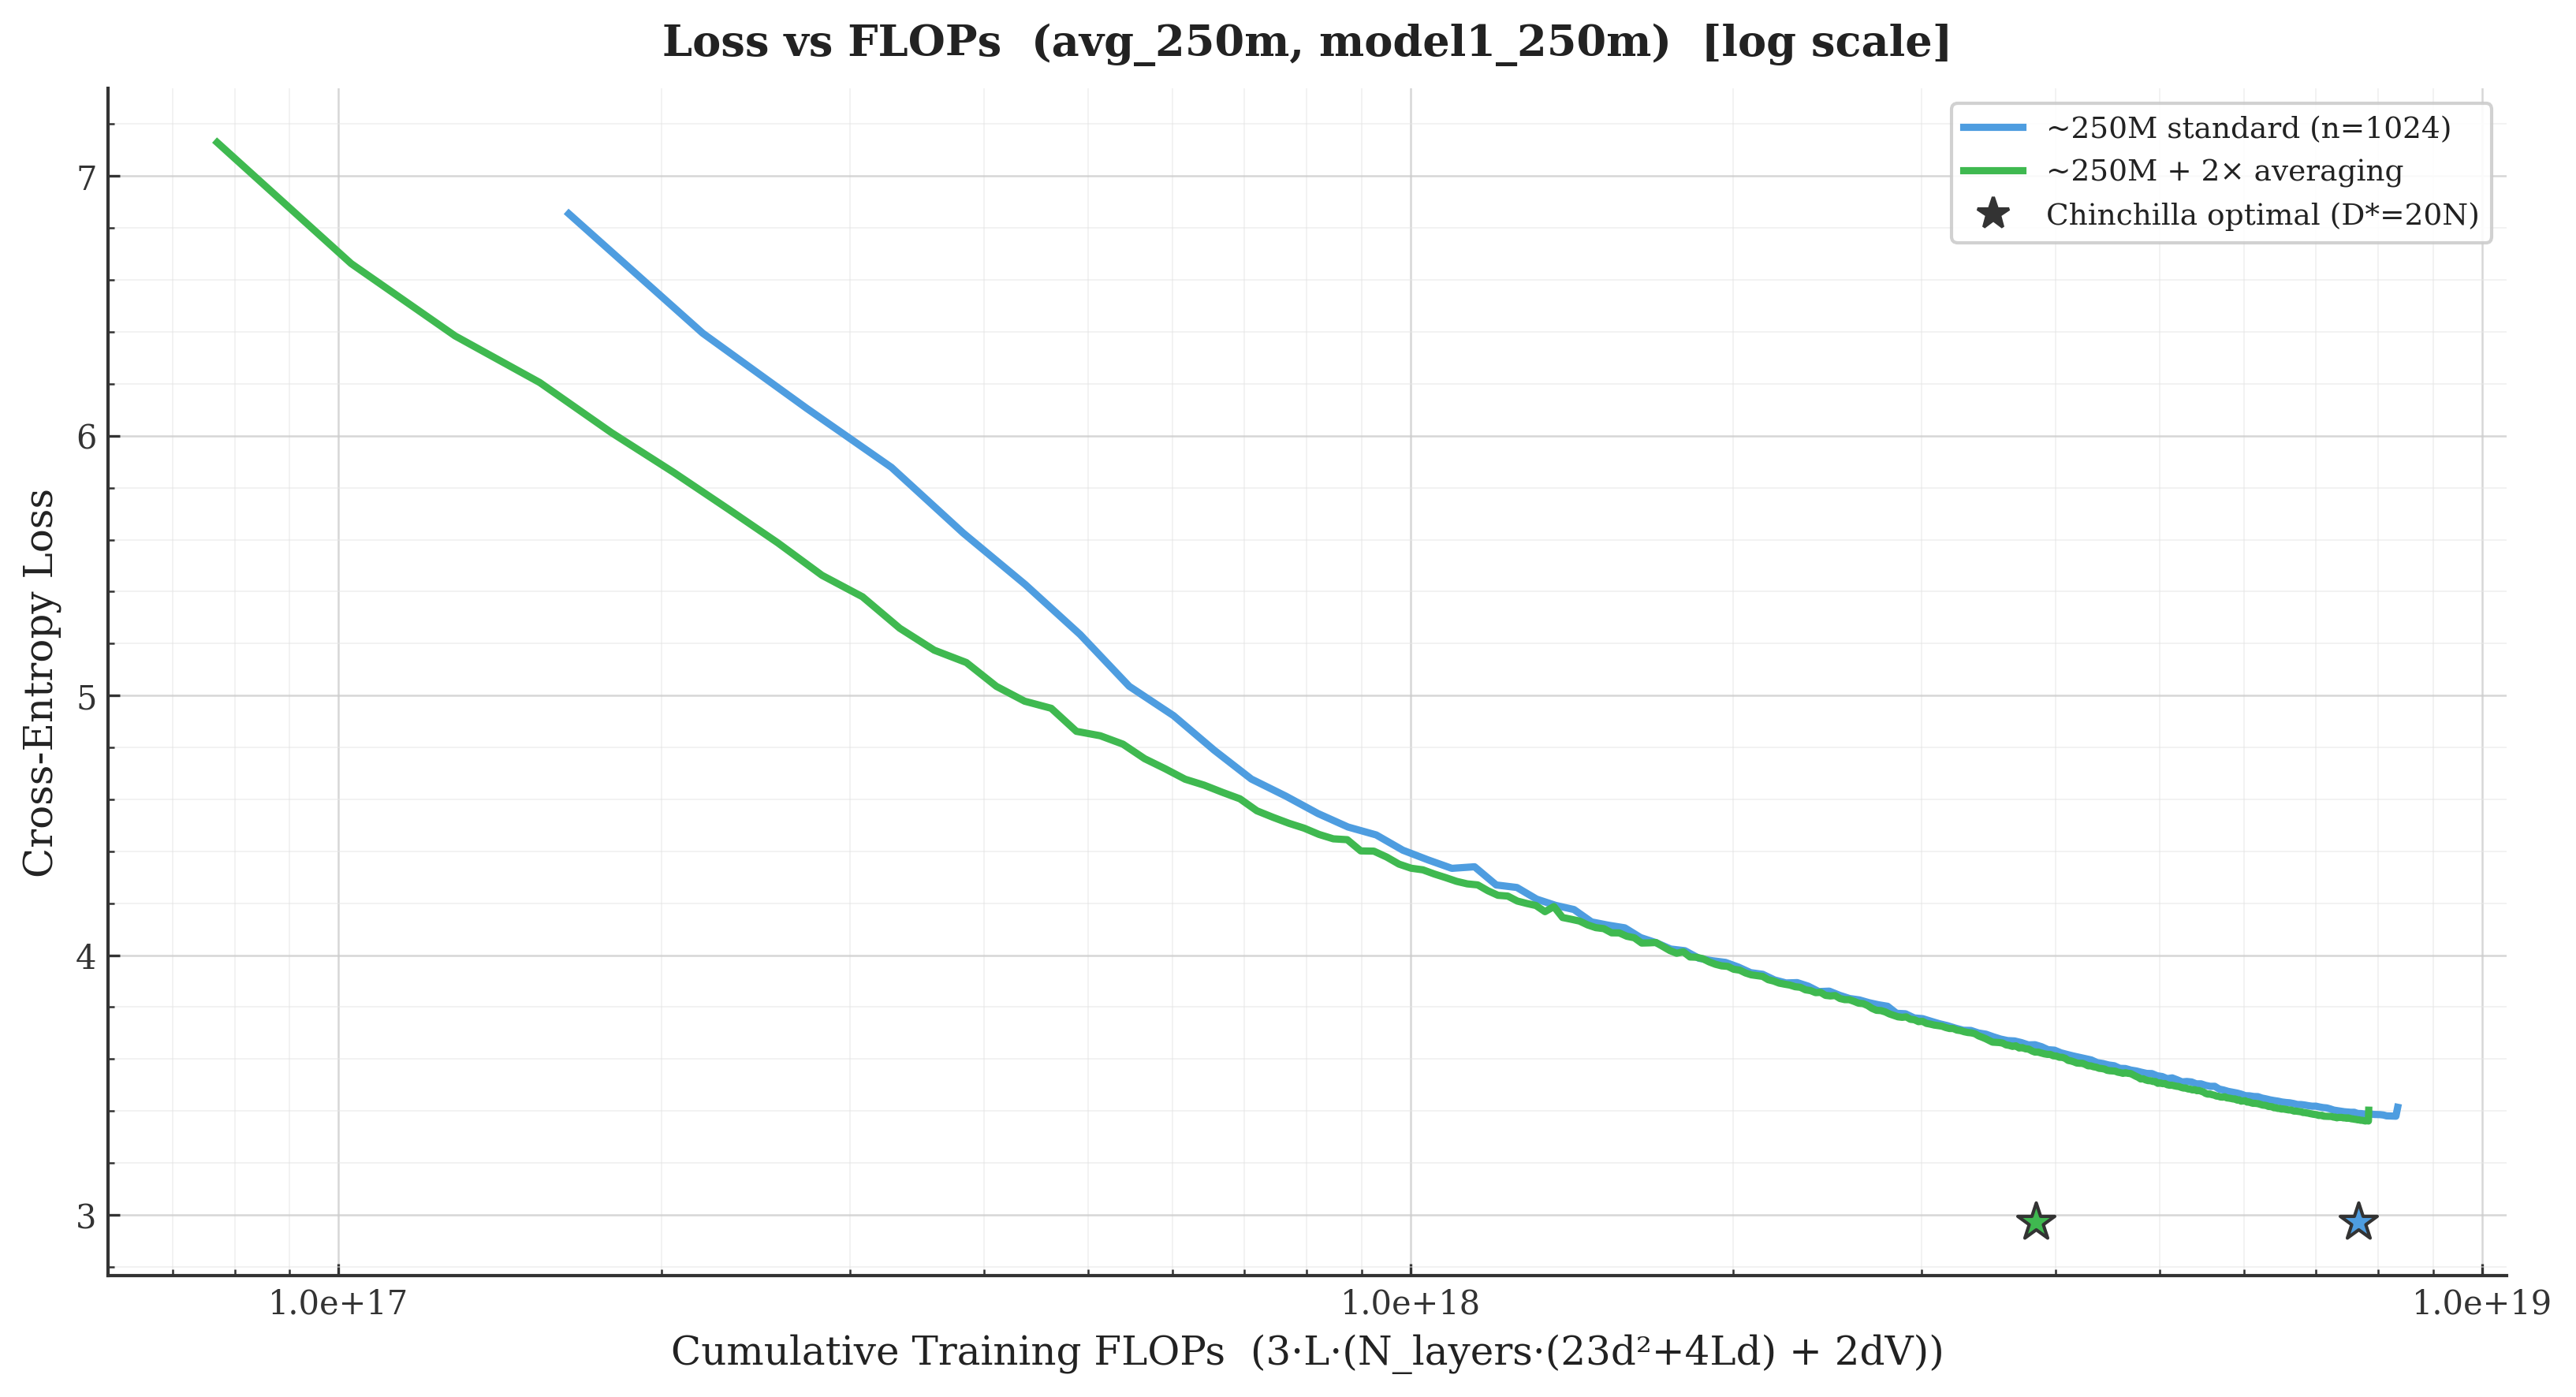
\includegraphics[width=\textwidth]{250m_loss_vs_flops_log.png}
    \caption{Loss vs.\ training FLOPs (log $x$).}
  \end{subfigure}\hfill
  \begin{subfigure}[b]{0.49\textwidth}
    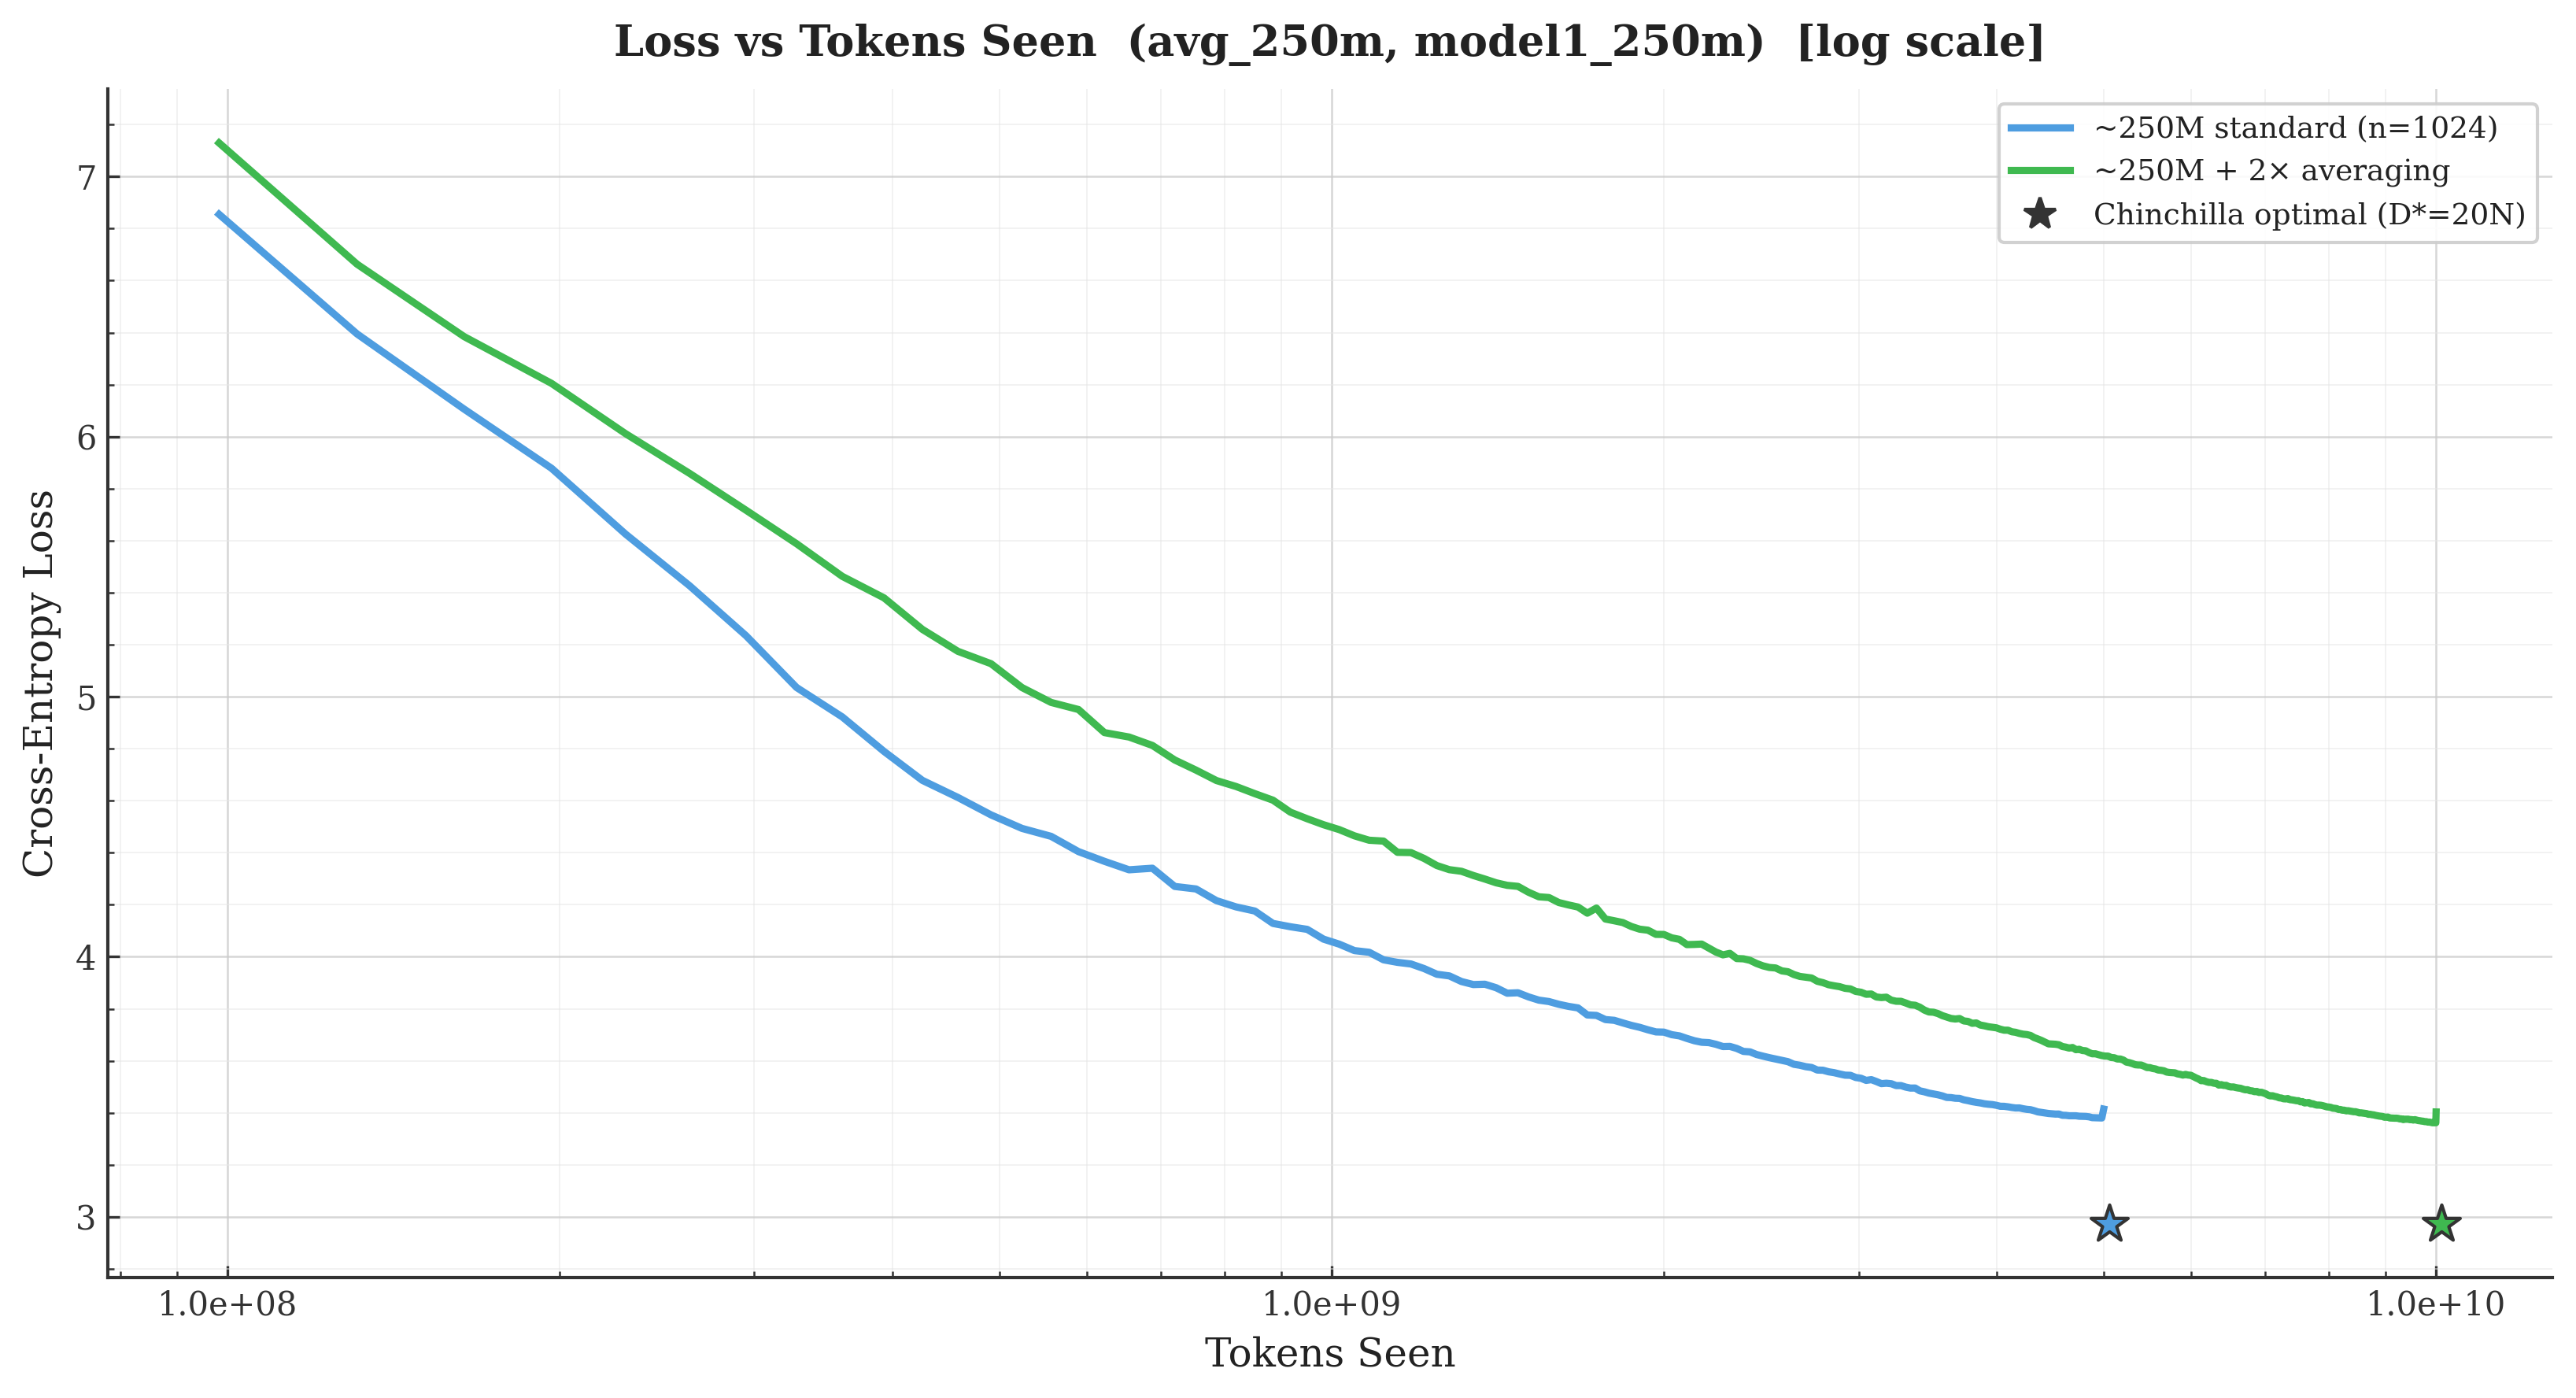
\includegraphics[width=\textwidth]{250m_loss_vs_tokens_log.png}
    \caption{Loss vs.\ raw tokens seen (log $x$).}
  \end{subfigure}
  \caption{250M comparison on native eval losses, both arms at their full
  budgets (5B and 10B raw tokens). The picture matches the smaller scales: the
  $k{=}2$ curve sits below the baseline at equal FLOPs throughout, and slightly
  above it on the raw-token axis.}
  \label{fig:250m}
\end{figure}

\begin{figure}[t]
  \centering
  \begin{subfigure}[b]{0.49\textwidth}
    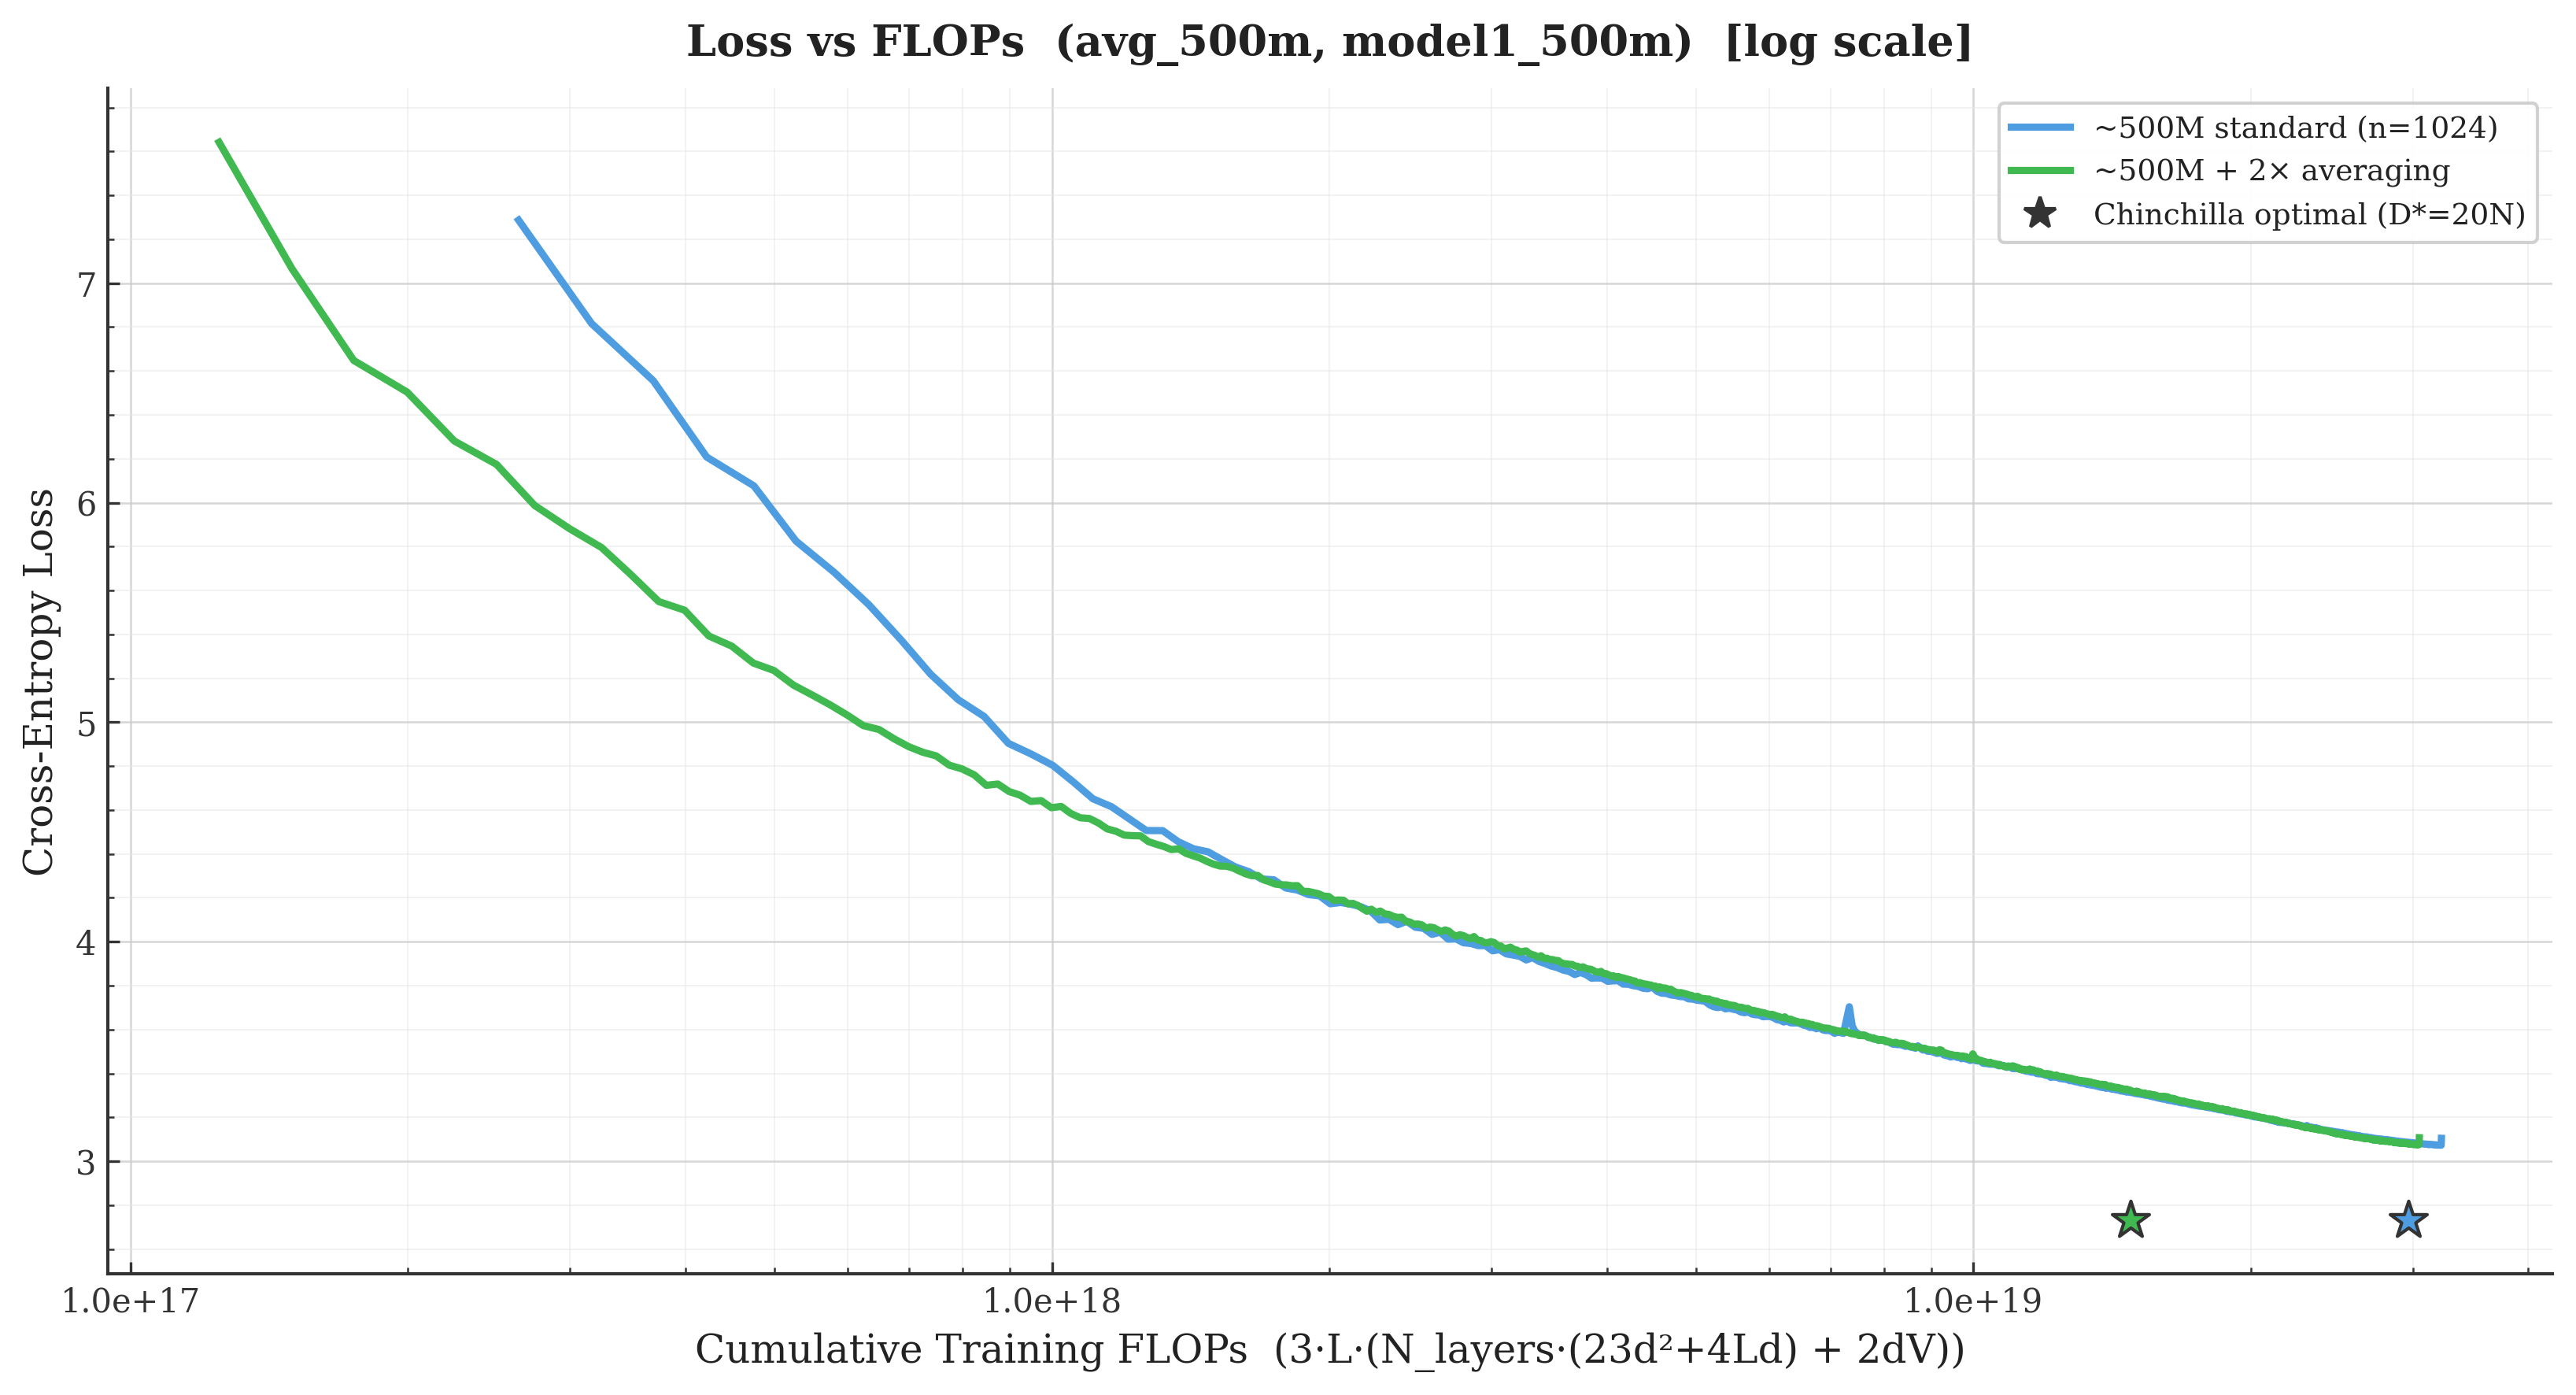
\includegraphics[width=\textwidth]{500m_loss_vs_flops_log.png}
    \caption{Loss vs.\ training FLOPs (log $x$).}
  \end{subfigure}\hfill
  \begin{subfigure}[b]{0.49\textwidth}
    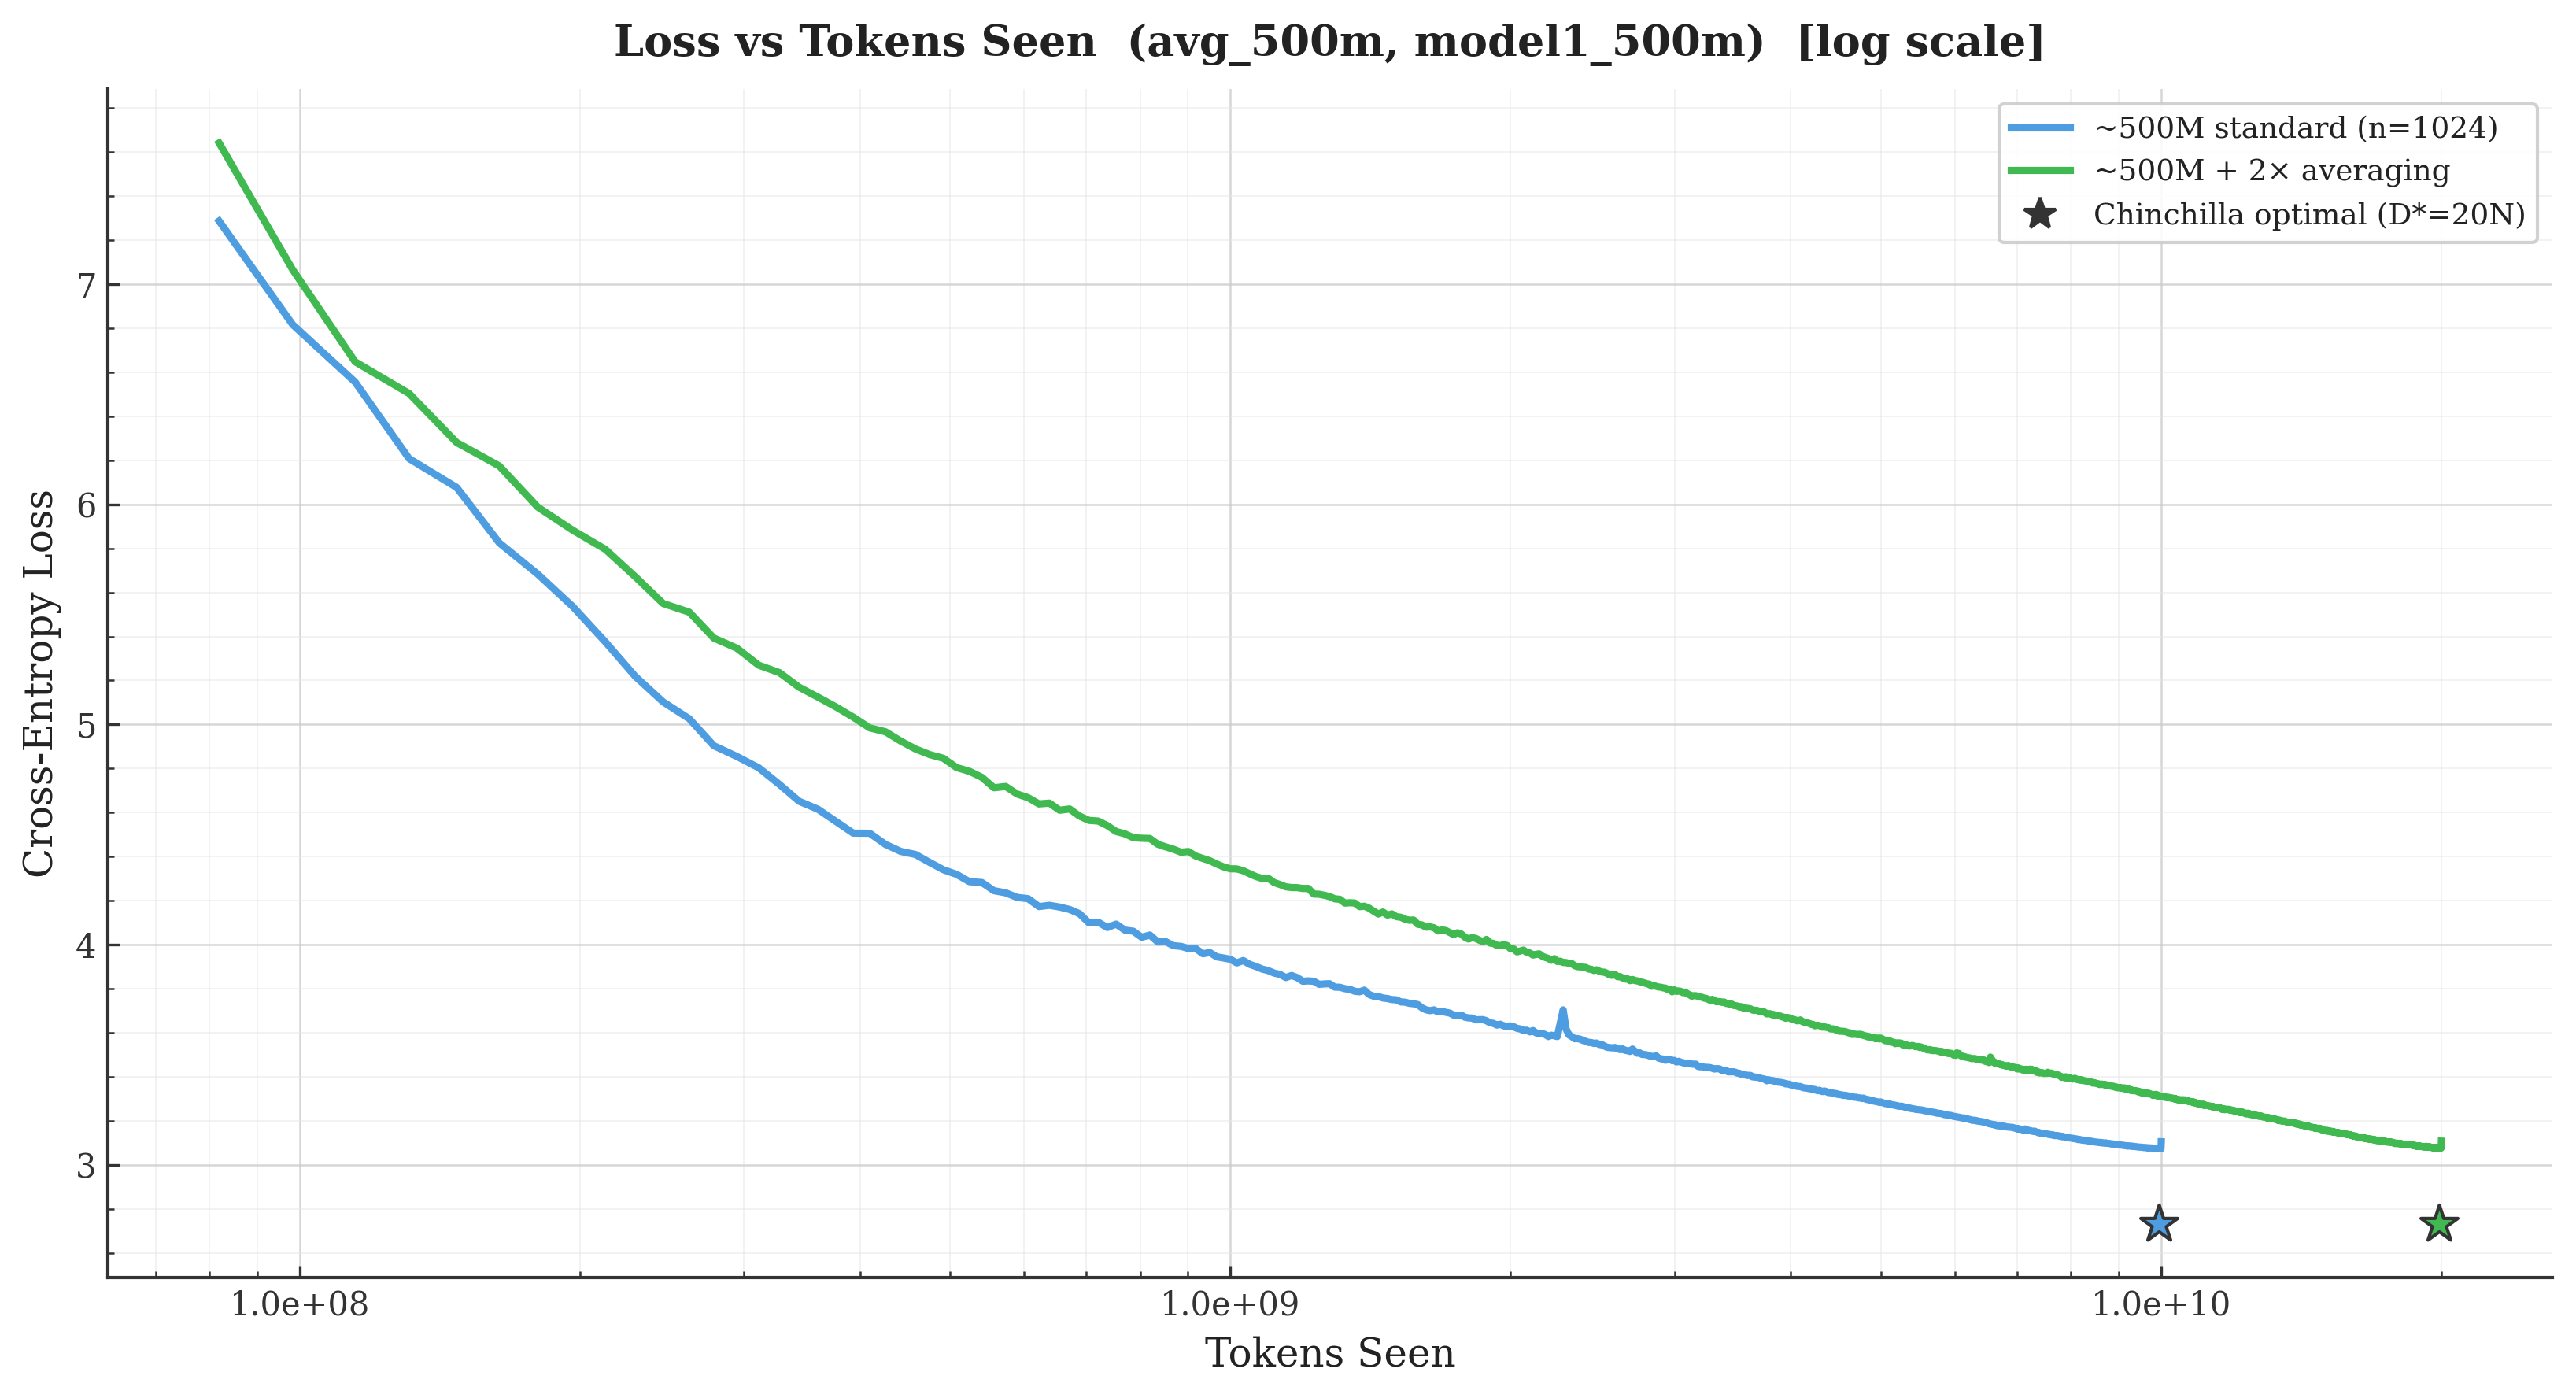
\includegraphics[width=\textwidth]{500m_loss_vs_tokens_log.png}
    \caption{Loss vs.\ raw tokens seen (log $x$).}
  \end{subfigure}
  \caption{500M comparison on native eval losses, both arms at their full
  budgets (10B and 20B raw tokens). The two FLOPs-axis curves are
  indistinguishable over the final decade of training and finish a few
  thousandths of a nat apart. The raw-token panel shows the same mechanism as
  at the smaller scales, with the averaged model below the baseline in compute
  but above it per token. A single isolated spike in the baseline's
  logged eval at step $69{,}000$, which recovers within one logging interval,
  is excluded from the plotted curve (Appendix~\ref{app:bugs}).}
  \label{fig:500m}
\end{figure}

\subsection{Full-position evaluation}
\label{sec:results-fullpos}

The curves above show native eval losses, which
Section~\ref{sec:offset-ensemble} argued do not compare like with like across
$k$. Table~\ref{tab:fullpos} rescores the final checkpoints with the
offset-ensemble protocol instead, so both arms are scored on identical
held-out sequences at identical target positions ($3{,}409{,}119$ predictions
per model at 125M).

The two scales in the table are measured slightly differently. The 125M rows
come from rescoring the saved checkpoints offline with
\texttt{eval\_full\_positions.py} over the full held-out set. The 500M rows
come from the same construction run inside the training loop, which we added
once random-offset training was in place so that later runs would not depend
on keeping checkpoints. It runs the averaged model once per offset
$o \in \{0,\dots,k-1\}$ and combines the resulting losses, weighted by how
many predictions each contributes. The construction is the same either way,
but the in-training version sees a smaller held-out sample, so the 500M
numbers are the noisier of the two.

\begin{table}[h]
\centering
\caption{Offset-ensemble full-position evaluation of the final more-data
checkpoints. Within each scale, both rows average over the identical set of
scored positions (every position $> k$ of each evaluation sequence), with the
baseline restricted to exactly the positions the $k{=}2$ ensemble covers. The
125M rows are offline rescorings over the full held-out set; the 500M rows are
the same construction computed in-training over a smaller sample.
\todo{fill 50M and 250M rows}}
\label{tab:fullpos}
\vspace{0.4em}
\begin{tabular}{llccc}
\toprule
Scale & Model & Mean NLL (nats/token) & PPL & Coverage \\
\midrule
125M & $k{=}1$ baseline (restricted) & 4.177 & 65.1 & all scored positions \\
125M & $k{=}2$, 2-offset ensemble & \good{\textbf{4.141}} & \good{\textbf{62.9}} & all scored positions \\
\midrule
500M & $k{=}1$ baseline (restricted) & 3.105 & 22.30 & all scored positions \\
500M & $k{=}2$, 2-offset ensemble & \good{3.102} & \good{22.25} & all scored positions \\
\midrule
50M & $k{=}1$ baseline (restricted) & \todo{} & & \\
50M & $k{=}2$, 2-offset ensemble & \todo{} & & \\
\midrule
250M & $k{=}1$ baseline (restricted) & \todo{} & & \\
250M & $k{=}2$, 2-offset ensemble & \todo{} & & \\
\bottomrule
\end{tabular}
\end{table}

At 125M the averaged model is better by $0.035$ nats, a \good{$3.4\%$
perplexity improvement}, while having spent $0.93\times$ the training FLOPs.
Both models are scored on the same positions here, each predicted once from
its full prefix, so this comparison does not have the problem the native
losses have.

At 500M the two arms finish level. The averaged model is $0.002$ nats ahead at
$0.946\times$ the training FLOPs, which is a $0.2\%$ perplexity difference.
That is too small to call a result. It comes from one unreplicated run, and it
is an order of magnitude below the $0.070$-nat spread we get at 50M just by
changing the training protocol (Section~\ref{sec:results-pooling}). We report
the pair and draw no conclusion from its sign. Settling it needs seed
replicates, which we have not yet run.
\todo{3 seeds at 500M with per-seed full-position NLL; report mean and
standard deviation so the sign at this scale can be stated with a confidence
interval rather than as a point estimate}

Splitting the 125M ensemble by offset confirms the argument of
Section~\ref{sec:offset-ensemble}. Offset 0 scores 4.145 and offset 1 scores
4.138, which is essentially equal, so no offset is privileged. That is what
random-offset training over packed data should produce, and it is what makes
the ensemble a faithful full-sequence likelihood rather than one
in-distribution pass mixed with $k{-}1$ out-of-distribution ones. Rotating
the offset during generation relies on the same property
(Appendix~\ref{app:offset}). Together, random-offset training and
offset-ensemble evaluation are what let patch-style training be a
\emph{final} operating point rather than a warm-up.

\subsection{Where the gain comes from: cheaper data, not longer context}
\label{sec:results-context}

There are two things averaging could be buying. One is more data per FLOP. The
other is more raw context behind each prediction, which averaging also makes
affordable. To tell them apart we trained four 50M models. All four are at
about equal compute except the full-attention control, which is deliberately
more expensive.

\begin{itemize}
  \item the baseline ($\Ltr{=}1024$, 1024 tokens of raw context);
  \item more-context $k{=}2$ (\texttt{seq\_len} 2048, $\Ltr{=}1024$, so
        $2\times$ the raw context at the same transformer cost);
  \item more-context $k{=}4$ (4096 tokens of raw context);
  \item a $k{=}1$ model with a genuinely 2048-token attention window, at
        $1.14\times$ the baseline's cost.
\end{itemize}

Native losses are comparable only within a fixed $k$ and grouping scheme, so
every comparison below is within one method: each longer-context arm against
the same-$k$ arm without the longer context.

\begin{table}[h]
\centering
\caption{Context experiment at 50M, native eval losses. The $\Delta$ column
compares each longer-context arm against the same-$k$ arm without the longer
context: $k{=}1$ full attention against the $k{=}1$ baseline; more-context
$k{=}2$ against more-data $k{=}2$ at 4.363; more-context $k{=}4$ against
more-data $k{=}4$ at 4.446. Losses in rows with different $k$ are not
comparable with each other.}
\label{tab:ctx}
\vspace{0.4em}
\small
\begin{tabular}{lccccc}
\toprule
Arm & Raw ctx & $\Ltr$ & Raw tokens & Train FLOPs & Final eval ($\Delta$ within method) \\
\midrule
$k{=}1$ baseline & 1024 & 1024 & 1.00B & $1.95\times10^{17}$ & \good{4.437} \\
$k{=}1$ full attention & 2048 & 2048 & 1.00B & $2.45\times10^{17}$ & 4.651 \;(\bad{$+0.214$}) \\
More context, $k{=}2$ & 2048 & 1024 & 2.00B & $1.95\times10^{17}$ & 4.650 \;(\bad{$+0.287$}) \\
More context, $k{=}4$ & 4096 & 1024 & 4.07B & $1.99\times10^{17}$ & 5.174 \;(\bad{$+0.728$}) \\
\bottomrule
\end{tabular}
\end{table}

Table~\ref{tab:ctx} and Figure~\ref{fig:ctx} give the result, and it is the
same in every comparison. \textbf{Longer raw context does not pay for itself at
this scale, in either method.} Within $k{=}1$, widening the attention window
from 1024 to 2048 costs $+0.214$ nats and $1.14\times$ the compute. Within
$k{=}2$, spending the averaging saving on doubled raw context (4.650) instead
of more data (4.363) costs $+0.287$ nats on the same prediction task. Within
$k{=}4$ the penalty grows to $+0.728$ nats.

This is a property of the data and the scale, not of averaging. Most FineWeb
documents are shorter than 1024 tokens, and packed sequences cross document
boundaries without masking, so context past 1024 tokens is mostly made up of
\emph{other documents'} text. The more context we add, the more of it is
irrelevant, which is why the penalty grows with the amount of extension.

That settles the question the experiment was built to answer. Extra context
does not help any of these arms, so the gains of the more-data setting are not
a context effect. On packed web text, what token averaging buys is data per
FLOP.

The experiment also answers the reverse question. When longer raw context is
what you actually want, averaging is the cheaper way to get it. The two
2048-context arms finish at the same loss (4.6503 for $k{=}2$ averaging, 4.6505
for full attention), but the averaged route spends $1.14\times$ less training
compute and holds half the KV cache and attention cost at inference for the
same raw context.
\todo{report the full-position endpoints for the two 2048-context arms here,
which is the comparable statement of this equality} This matters most on data
where long context genuinely helps, such as long documents or code, which we
leave to follow-up work. \todo{loss-vs-position curves; document-length
distribution of FineWeb; PG19/code long-context experiment}

\begin{figure}[t]
  \centering
  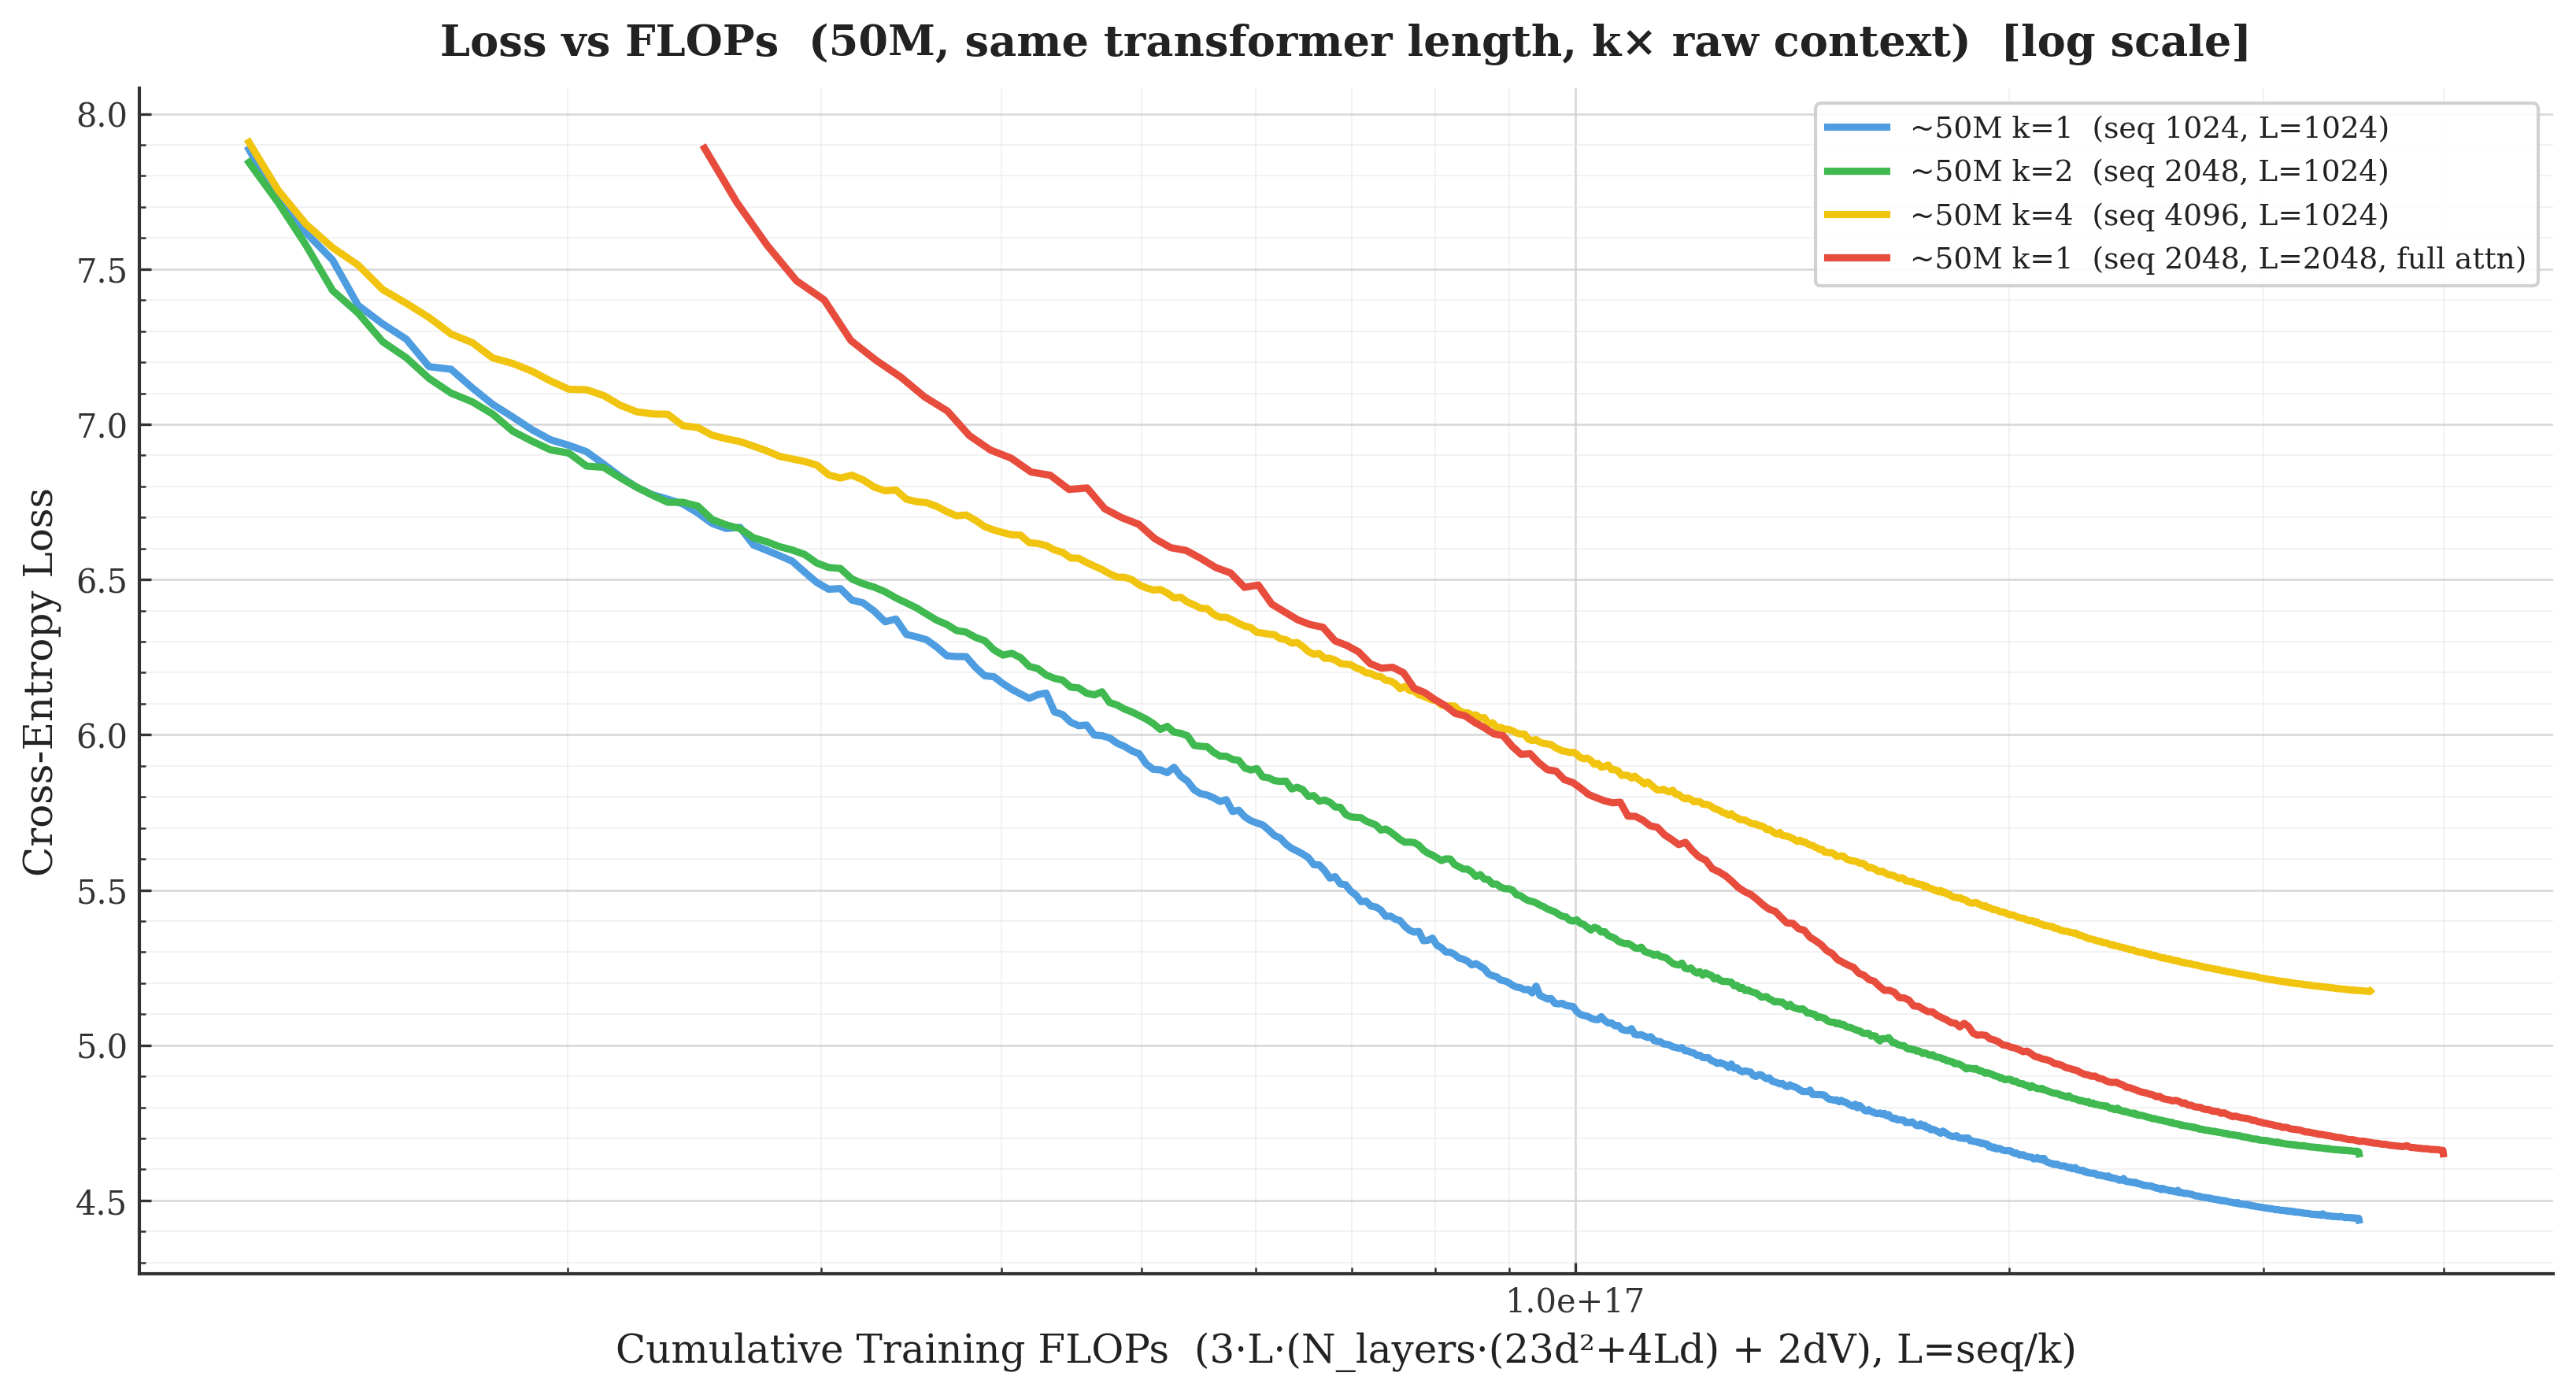
\includegraphics[width=0.75\textwidth]{50m_kx_ctx_loss_vs_flops_log.png}
  \caption{Context experiment at 50M: native eval loss vs.\ training FLOPs
  (log $x$). Curves with different $k$ score different sets of positions and
  are overlaid only for orientation; the valid comparisons are within one
  method (see text). The two arms with 2048 tokens of raw context (green:
  $k{=}2$ averaging; red: full attention) end at almost the same native loss
  at very different cost, and $4\times$ context (yellow) is worse still.
  Early-training loss spikes are clipped at 8.0 for readability.}
  \label{fig:ctx}
\end{figure}

\subsection{Pooling functions: weighting by content and position beats the
mean}
\label{sec:results-pooling}

Everything the transformer learns passes through the pooling function, so we
compared the six functions of Section~\ref{sec:method-pooling} at 50M in the
more-data setting. All six runs use one matched protocol. Architecture, data,
batch size, update schedule, warmup, embedding tying and evaluation are
identical, and the token budget is fixed within each $k$ (2.00B raw tokens at
$k{=}2$, 4.07B at $k{=}4$). Within each $k$ block the runs share the same $k$
and, apart from the word-aligned one, the same grouping scheme, so their native
losses can be compared with each other. Figure~\ref{fig:pooling} shows all the
curves and Table~\ref{tab:pooling} the final and quarter-budget losses.

One comparison does not hold. The word-aligned variant predicts a different
distribution of positions (word starts only) at a slightly different realized
compression, so its native loss is not measured on the same prediction task as
the fixed-size variants. We report it as indicative and leave it out of the
ordering (Appendix~\ref{app:word}).

\begin{figure}[t]
  \centering
  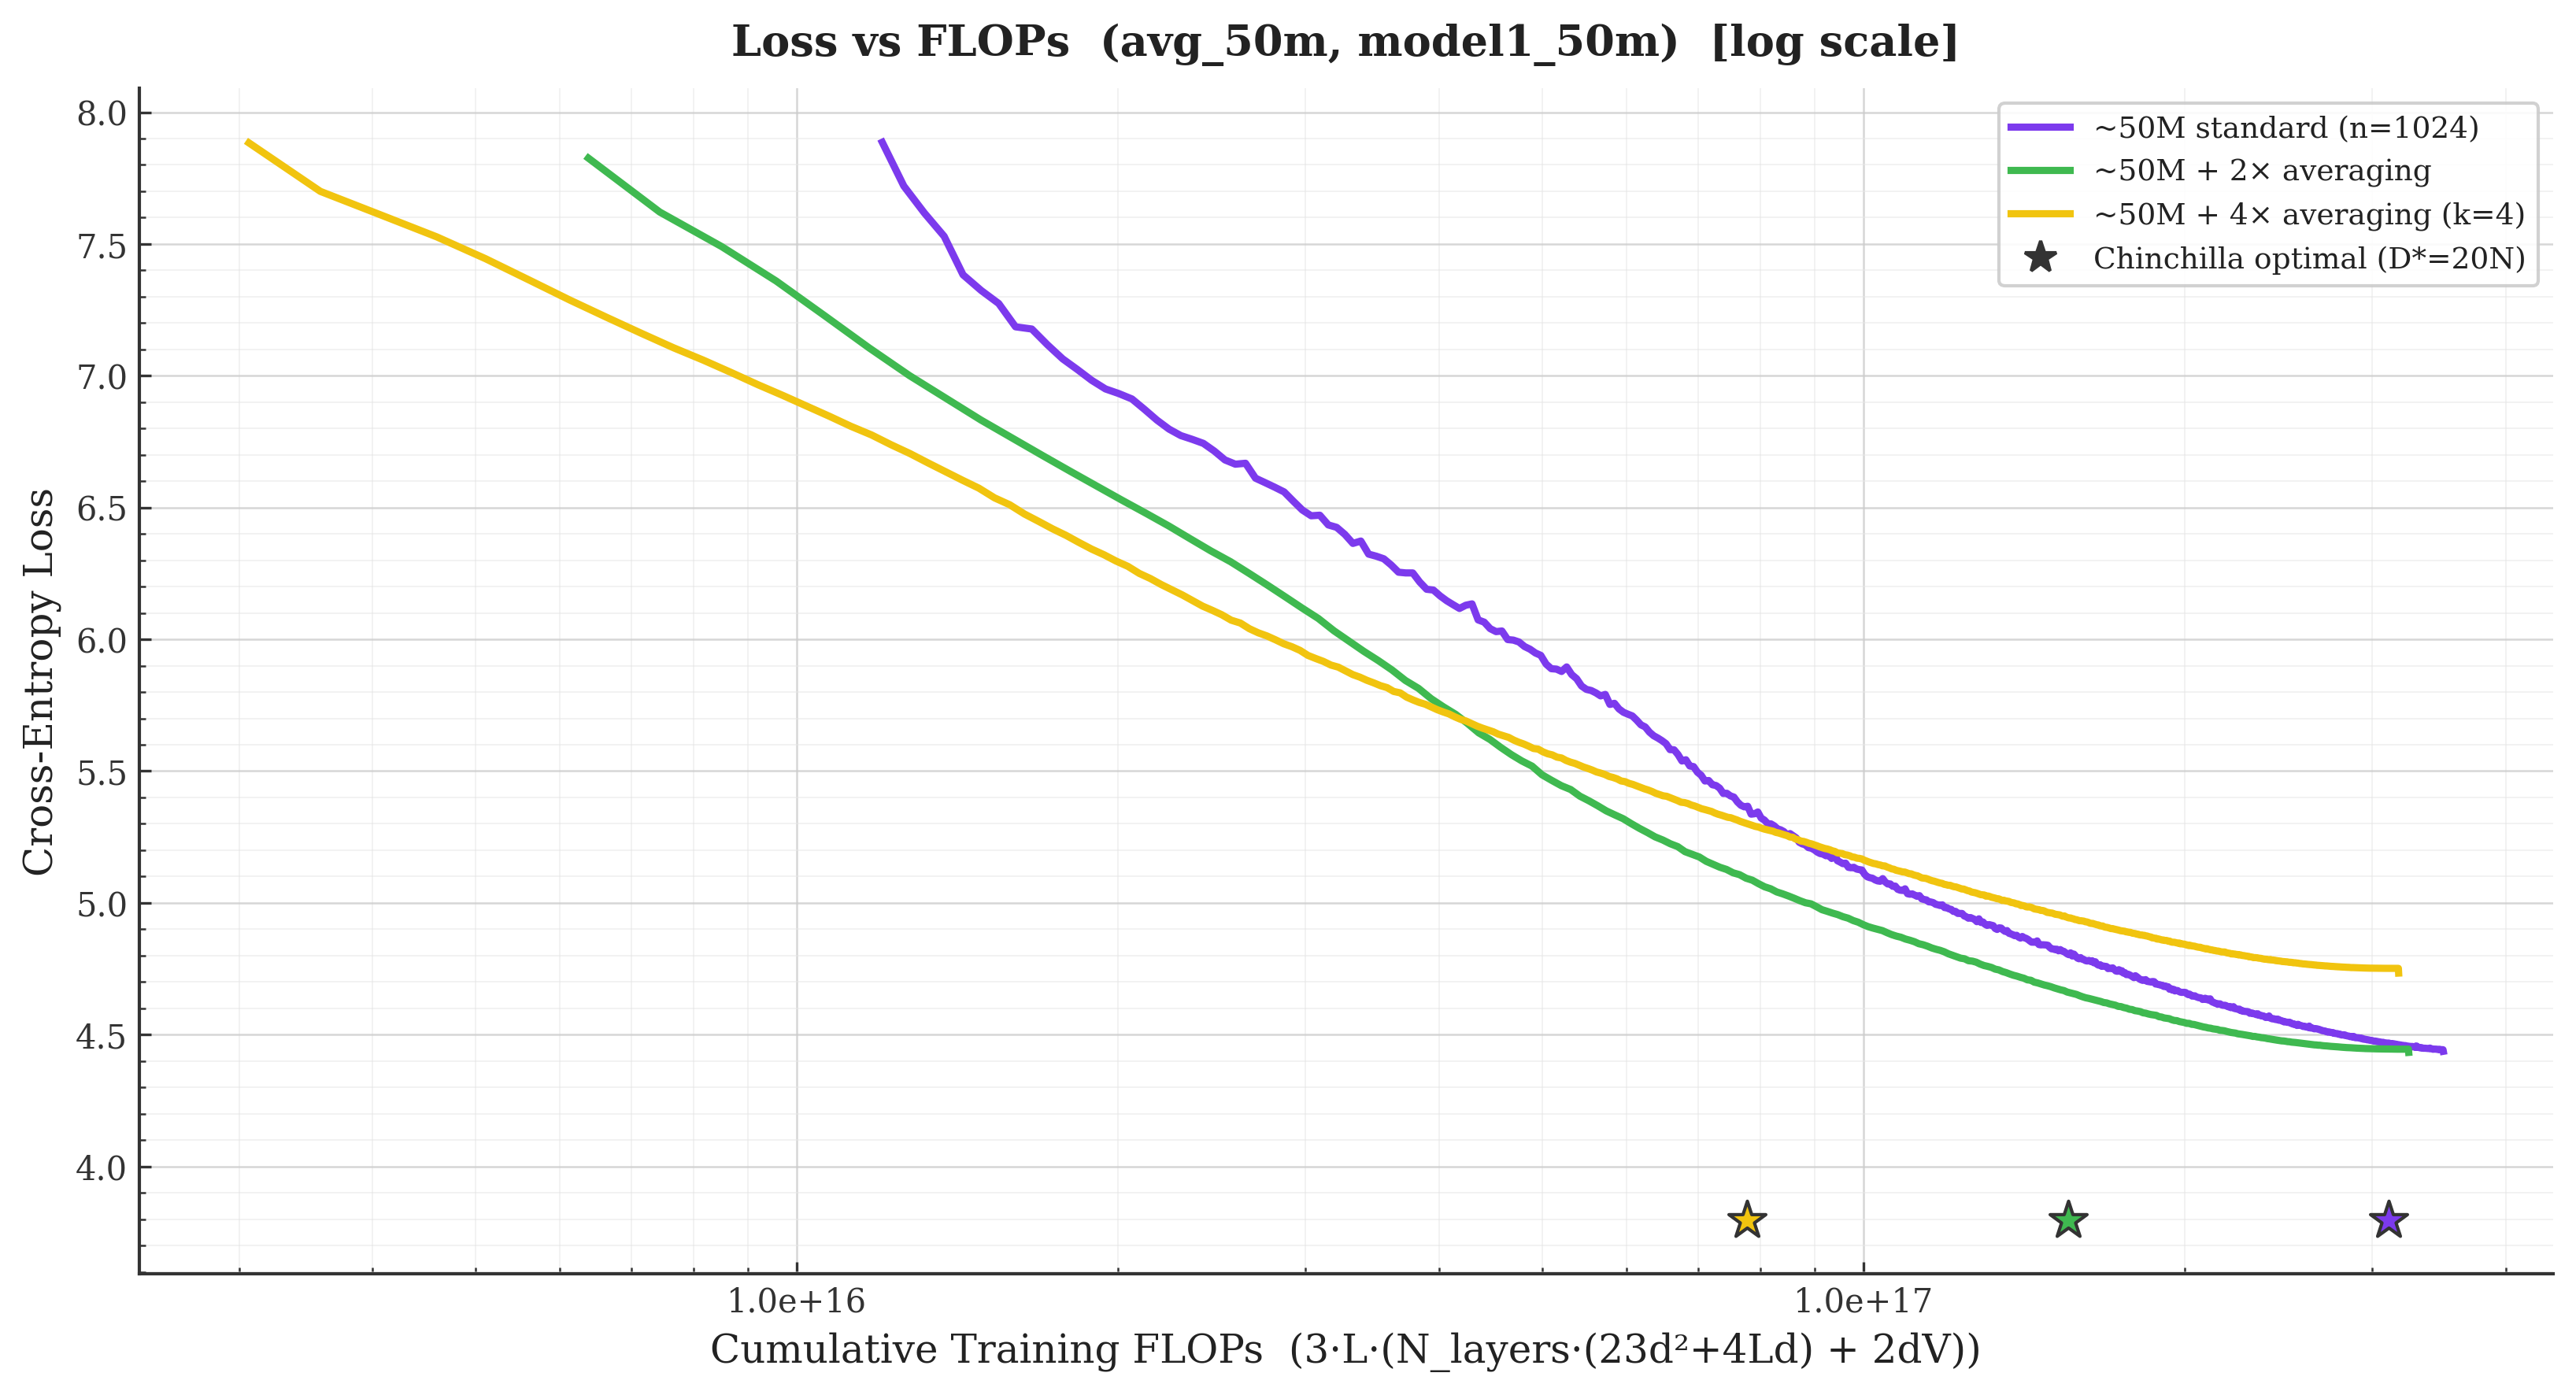
\includegraphics[width=0.8\textwidth]{50m_loss_vs_flops_log.png}
  \caption{Pooling functions at 50M: native eval loss vs.\ recomputed training
  FLOPs (log $x$), with all $k{=}2$ and $k{=}4$ variants overlaid on the
  $k{=}1$ baseline and the original mean-pooling runs. Curves are comparable
  with each other only within one $k$ block and one protocol; see text.}
  \label{fig:pooling}
\end{figure}

\begin{table}[h]
\centering
\caption{Pooling functions at 50M in the more-data setting, under one matched
protocol. Native eval CE (nats/token) at the nearest logged checkpoint to each
quarter of the token budget. Runs are comparable within a $k$ block; the
word-aligned row is measured on a different prediction task
(Appendix~\ref{app:word}). Every entry is a single run at one seed.
\todo{add variance bars once the seed replicates specified in
Section~\ref{sec:results-pooling} are available}}
\label{tab:pooling}
\vspace{0.4em}
\small
\begin{tabular}{llccccc}
\toprule
$k$ & Pooling & 25\% & 50\% & 75\% & Final & Final PPL \\
\midrule
2 & \good{\textbf{learned: content + position}} & 5.170 & 4.619 & 4.389 & \good{\textbf{4.326}} & \good{\textbf{75.7}} \\
2 & mean & 5.174 & 4.649 & 4.425 & 4.363 & 78.5 \\
2 & learned: content only & 5.222 & 4.675 & 4.443 & 4.383 & 80.1 \\
2 & overlapping groups ($w{=}4, s{=}2$) & 5.460 & 4.820 & 4.562 & 4.492 & 89.3 \\
2 & word-aligned (task differs) & 5.413 & 4.872 & 4.640 & 4.577 & 97.2 \\
2 & fixed recency & 5.439 & 4.962 & 4.707 & 4.617 & 101.2 \\
\midrule
4 & \good{\textbf{learned: content + position}} & 4.951 & 4.463 & 4.224 & \good{\textbf{4.163}} & \good{\textbf{64.3}} \\
4 & fixed recency & 5.041 & 4.569 & 4.330 & 4.265 & 71.1 \\
4 & learned: content only & 5.315 & 4.753 & 4.512 & 4.445 & 85.2 \\
4 & mean & 5.326 & 4.756 & 4.505 & 4.446 & 85.2 \\
\bottomrule
\end{tabular}
\end{table}

\paragraph{One rule leads at both compression ratios.}
The pooler that weights tokens by content and position gives the lowest native
loss at both $k{=}2$ and $k{=}4$, and it is the only rule whose standing holds
up at both. The two fixed rules swap places: the plain mean is second best at
$k{=}2$ and last at $k{=}4$, while the fixed recency weighting is last at
$k{=}2$ and second best at $k{=}4$. At $k{=}2$ the learned pooler
finishes $0.037$ nats ahead of the mean, and it is ahead at every
quarter-budget checkpoint. At $k{=}4$ its margin over the mean grows to $0.283$
nats, which is $0.102$ ahead of the next-best rule, the fixed recency
weighting, and again it leads at every checkpoint. It costs $\dmodel + 1 + k$
parameters, which is negligible at any scale.

Every entry in Table~\ref{tab:pooling} is a single run at one seed, so these
are observed orderings rather than established ones. At $k{=}4$ the $0.283$-nat
margin is too large for seed noise to explain. At $k{=}2$ the $0.037$-nat margin
is not, and we do not yet have the replicates to bound it. Being ahead at every
quarter-budget checkpoint is weaker evidence than independent seeds would be,
because checkpoints within one run are strongly correlated.
\todo{SEED REPLICATES (planned; the single owner of every seed/variance
claim in this paper, other seed notes point here).
\emph{Runs:} \texttt{avg\_50m\_k2\_learnable\_pos} and
\texttt{avg\_50m\_k2} (matched mean) at 2 additional seeds each, i.e.\ 4
runs of 2B raw tokens under the matched protocol
(16{,}384 raw tokens/update, tied embeddings, 2k warmup), for
${\sim}1.3\times10^{18}$ total FLOPs. Optionally add
\texttt{avg\_50m\_k4\_learnable\_pos} and \texttt{avg\_50m\_k4} at 1
additional seed each to confirm the $k{=}4$ margin, though $0.283$ nats is
unlikely to be seed noise.
\emph{Report:} per-variant mean and standard deviation of final native
eval loss, and the seed spread of the learnable+pos minus mean difference
at $k{=}2$. If that spread is comparable to $0.037$ nats, downgrade the
$k{=}2$ ordering to ``indistinguishable'' in the abstract, the Findings
list, Table~\ref{tab:pooling}, and this section.
\emph{Then remove:} this paragraph's hedging, the variance caveat in
Table~\ref{tab:pooling}'s caption, and the seed note in
Appendix~\ref{app:runs}.}

\paragraph{What the mean seems to miss is position, not content.}
The remaining rows show where the win comes from. At $k{=}4$, the
\emph{fixed} recency weighting on its own recovers most of the gap to the
leader (4.265 against 4.446 for the mean), while the scorer that sees only
content recovers none of it (4.445, indistinguishable from the mean).

One confound has to be stated before reading that causally. At $k \geq 4$ we
initialize the content-plus-position pooler's position logits \emph{at} the
exponential recency rule, while the content-only scorer is zero-initialized and
so starts at plain mean pooling. Part of the $k{=}4$ separation between the two
learned poolers therefore comes from where they start rather than from what
they can express, and a clean test would initialize both the same way. At
$k{=}2$ both start uniform, so that comparison is free of the confound, and
there the position term still helps. The fixed-weighting rows do not depend on
initialization at all, and they point the same way.

The likely explanation is architectural. The content scorer looks at each
embedding on its own, before the network has any positional signal, so it
cannot express ``the last token of the group matters most''. That prior is
worth a lot when four tokens collapse into one vector, because the group's last
token is the one next to the prediction target.

At $k{=}2$ the same prior hurts when applied as an aggressive fixed rule. The
fixed recency weighting gives 4.617 there, the worst result we measured. With
only two tokens per group both carry useful signal, and systematically
down-weighting the first throws that away. The content-plus-position pooler
does better at both ratios because it learns how much to favour later slots
instead of having that fixed in advance, and the content term then adds a
little more on top.

The structural alternatives point away from the other explanations we
considered. Overlapping groups remove hard boundary cuts entirely and
word-aligned groups make each group a whole word, and both do worse than the
plain mean. So neither boundary effects nor linguistically meaningful grouping
looks like the main thing at work.

\paragraph{Why the matched protocol matters.}
Training details move the results by more than the pooling functions do. Mean
pooling trained under our earlier protocol (${\sim}8\times$ fewer optimizer
updates for the same token budget, and correspondingly different warmup
exposure) ends $0.070$ nats worse at $k{=}2$ and $0.288$ nats worse at $k{=}4$
than the same model under the matched protocol. The update schedule alone
therefore moves final losses by more than most of the gaps in
Table~\ref{tab:pooling}. That is why every pooling function in this section is
trained under one identical protocol, and why we keep the older mean-pooling
runs in Appendix~\ref{app:runs} as references only and never use them as
controls.
\todo{offset-ensemble rescoring of the pooling winners; learned weight
profiles (Appendix~\ref{app:pooling}); seeds are specified in the seed
replicate note above}

% =====================================================================
\section{Discussion and Limitations}
% =====================================================================
\label{sec:limitations}

\paragraph{Scale.}
Every equal-loss saving we can measure comes from the 50M--250M range, a factor
of five in parameters. At 500M the two arms finish level and we cannot measure
a saving there at all. Whether averaging still helps at 500M and above is the
largest open question in the paper, and answering it needs two things we have
not done: seed replicates at 500M, so that the sign at that scale gets a
confidence interval instead of being a single point, and the 1B pair.

Data logistics are part of the difficulty. The $k{=}2$ arm consumes twice the
raw tokens, and the 250M $k{=}2$ run already exhausts FineWeb sample-10BT, so
the 500M pair and everything above it draws from \texttt{sample-100BT}. We
change the slice for both arms of a scale, so no within-scale comparison is
affected. \todo{1B results; seed replicates at 500M}

\paragraph{Tokenizer granularity.}
Averaging two tokens looks a little like using a tokenizer whose tokens are
twice as long. The two are not the same, because averaging keeps the fine
vocabulary and composes embeddings on the fly, but the direct control is a
coarser-tokenizer baseline compared in bits-per-byte.
\todo{coarser-tokenizer baseline in bits-per-byte}

\paragraph{Generation and downstream evaluation.}
Everything we report is language-modeling loss. Rotating-offset decoding
(Appendix~\ref{app:offset}) gives token-by-token generation at about the cost of
an ordinary decoder, and downstream zero-shot results (LAMBADA, HellaSwag, PIQA,
ARC-E) are the natural complement to the loss numbers. A small local decoder
that emits all $k$ tokens of a group, in the style of Block Transformer, would
give native generation and is a further extension.
\todo{rotating-offset decoding benchmark; downstream evals}

\paragraph{How far the context result generalizes.}
Our finding that longer raw context hurts is a statement about packed FineWeb at
these scales, where most documents are shorter than 1024 tokens and packing
crosses document boundaries without masking. It is not a claim about
long-document corpora, code, or masked packing. On those, the fact that
averaging buys context more cheaply than full attention could turn into a
genuine long-context win. We think this is the most promising unexplored part of
the work.

% =====================================================================
\section{Conclusion}
% =====================================================================
\label{sec:conclusion}

\todo{Write after the 1B endpoints and the remaining full-position numbers
land. Skeleton: (i) token averaging turns cheap data into lower loss at fixed
compute, giving $3.4\%$ lower perplexity at $0.93\times$ the FLOPs on the
comparable metric at 125M and equal-loss compute savings of $1.48\times$ at
50M, $1.43\times$ at 125M and $1.31\times$ at 250M, with the 500M pair
finishing level, so the benefit at larger scale is unresolved pending 500M
replicates and the 1B pair; (ii) random-offset
training and offset-ensemble evaluation solve the comparability problem and let
patch-style operation be a final operating point, with rotating-offset decoding
for generation; (iii) longer raw context hurts on packed web text, so the gain
is cheaper data, while averaging is the cheaper way to buy context when context
is what you want; (iv) weighting tokens by content and position is the best
pooling rule at both compression ratios, and position is the ingredient the mean
discards. Close with the scaling question as the decisive open item.}

% =====================================================================
\section*{References}
% =====================================================================
\todo{complete bibliography when Related Work is written}

\noindent\hangindent=1.5em\hangafter=1
Hoffmann, J., Borgeaud, S., Mensch, A., Buchatskaya, E., Cai, T.,
Rutherford, E., de Las Casas, D., Hendricks, L.~A., Welbl, J., Clark, A.,
Hennigan, T., Noland, E., Millican, K., van den Driessche, G., Damoc, B.,
Guy, A., Osindero, S., Simonyan, K., Elsen, E., Rae, J.~W., Vinyals, O., \&
Sifre, L. (2022). Training compute-optimal large language models.
\emph{arXiv preprint arXiv:2203.15556}.

% =====================================================================
\appendix
% =====================================================================

\section{FLOPs Derivation}
\label{app:flops}

Per layer and per transformer position, counting multiply--accumulates as 2
FLOPs, forward pass:
\begin{itemize}
  \item Attention projections: $Q, K, V$, and output, i.e.\ four $d \times
        d$ matmuls: $4 \times 2d^2 = 8d^2$.
  \item SwiGLU FFN with \texttt{ff\_multiplier} 2.5: the combined
        implementation projects $d \to 5d$ for up and gate ($2 \cdot 5d^2 =
        10d^2$), then projects down $2.5d \to d$ ($2 \times 2.5 d^2 =
        5d^2$): total $15d^2$. (A standard $4\times$ FFN would give
        $16d^2$; our architecture's SwiGLU at 2.5 gives $15d^2$, and we use
        the exact value.)
  \item Attention scores and value aggregation: $2 \cdot 2 \Ltr d = 4\Ltr d$
        per position at sequence length $\Ltr$ (causal masking halves the
        effective term; we follow the standard convention of quoting the
        full-matrix count and apply it uniformly to all arms, so ratios are
        unaffected). \todo{state the causal-mask convention once and verify
        consistency with plotting code}
  \item Output projection: one $d \to V$ matmul per scored position,
        $2dV$, with $V = 50{,}304$. Each transformer position emits exactly
        one prediction in both arms, so this term is proportional to
        $\Ltr$ and not to \texttt{seq\_len}.
\end{itemize}
Total forward: $n_{\mathrm{layers}}(23d^2 + 4\Ltr d) + 2dV$ per position.
Training multiplies by 3 (forward + backward). A sequence of
\texttt{seq\_len} raw tokens occupies $\Ltr = \texttt{seq\_len}/k$ positions,
which gives Eq.~\eqref{eq:flops}. Every plot and table in this paper computes
FLOPs from \texttt{tokens\_seen} through that equation.

The output projection is a large share of the total at these scales rather than
a correction term, so we tabulate it explicitly. As a fraction of the baseline
arm's total training FLOPs it is $44.2\%$ at 50M ($d{=}512$), $27.8\%$ at 125M
($d{=}768$) and $18.5\%$ at 250M ($d{=}1024$), falling as $d$ grows towards $V$.
Both arms score one token per transformer position, and the equal-compute design
gives them equal position counts, so in absolute terms this term contributes
\emph{equally} to both. Including it therefore moves every efficiency ratio
towards $1$: the final cost ratios are $0.928/0.932/0.940$ with the head and
would be $0.871/0.906/0.926$ without it, and the equal-loss multipliers are
$1.48/1.43/1.31$ with the head and $1.58/1.47/1.33$ without. The
head-exclusive figures do not describe total training cost, so we do not report
them as though they did.

We exclude input embedding lookups on both arms. The lookup is a gather rather
than a matmul, and the averaged arm performs $k\times$ as many of them per
transformer position, so leaving it out is the conservative choice for the
method.

\section{Equal-Loss Compute Saving: How We Read It}
\label{app:equalloss}

The equal-loss savings quoted in Section~\ref{sec:results-main} are measured
off the logged curves, not fitted or extrapolated. The procedure for one
$(k{=}1, k{=}2)$ pair is:

\begin{enumerate}
  \item Take the target loss $L^\ast$ to be the baseline's eval loss at its
        last logged step, and $C_{\mathrm{base}}$ to be that run's total
        training FLOPs.
  \item Walk along the averaged run's logged evaluations and find the first
        one whose loss is at or below $L^\ast$. Interpolate linearly between
        that point and the one before it, in $(\log C, \text{loss})$ space, to
        get $C_{\mathrm{avg}}$, the compute at which the averaged run first
        reaches $L^\ast$.
  \item Report $C_{\mathrm{base}} / C_{\mathrm{avg}}$.
\end{enumerate}

FLOPs are recomputed from \texttt{tokens\_seen} through Eq.~\eqref{eq:flops}
in both runs; the \texttt{cumulative\_flops} column written by the training
loop is ignored. Duplicate steps from resumed runs are dropped, keeping the
last record for each step. Table~\ref{tab:equalloss} gives the inputs and the
result at each scale. The script that produces it is
\texttt{experiments/chinchilla/equal\_loss\_saving.py}.

\begin{table}[h]
\centering
\caption{Inputs to each equal-loss reading. $L^\ast$ is the baseline's final
eval loss. $C_{\mathrm{avg}}$ is where the averaged run's curve crosses it.
Losses are native eval losses, with the caveat of
Section~\ref{sec:results-main}. The 50M averaged arm is the matched-protocol
run of Section~\ref{sec:results-pooling}.}
\label{tab:equalloss}
\vspace{0.4em}
\begin{tabular}{lcccc}
\toprule
Scale & $L^\ast$ & $C_{\mathrm{base}}$ & $C_{\mathrm{avg}}$ & Saving \\
\midrule
50M  & 4.437 & $3.50\times10^{17}$ & $2.36\times10^{17}$ & \good{$1.48\times$} \\
125M & 4.204 & $2.08\times10^{18}$ & $1.46\times10^{18}$ & \good{$1.43\times$} \\
250M & 3.414 & $8.34\times10^{18}$ & $6.38\times10^{18}$ & \good{$1.31\times$} \\
500M & 3.105 & $3.22\times10^{19}$ & \multicolumn{2}{l}{not reported, see below} \\
\bottomrule
\end{tabular}
\end{table}

We do not report a 500M number because the reading is not stable there. The
two curves finish a few thousandths of a nat apart, so the answer depends on
which logged evaluation we read. Taking the baseline's last logged loss
($3.105$) as the target gives $1.21\times$. Taking the one before it
($3.073$) gives no answer at all, because the averaged run's curve never
reaches that loss: its own minimum over the whole run is $3.075$. A quantity
that swings between $1.21\times$ and unattainable across two adjacent
evaluations of the same run is not measuring a compute saving, so we leave it
out. Both runs also log a small upward step at their final evaluation
($3.073 \to 3.105$ for the baseline, $3.076 \to 3.107$ for the averaged arm),
which is a further reason to treat the endpoint reading at this scale with
care.

\section{Offset-Ensemble Evaluation: Details}
\label{app:offset}

For a $k$-averaged model and evaluation sequence $t_{1..T}$, offset $o \in
\{0, \dots, k{-}1\}$ discards the first $o$ tokens, forms $n_o = \lfloor
(T-o)/k \rfloor$ groups, embeds and pools them, and runs the transformer on the
first $n_o - 1$ compressed positions. The prediction at compressed position $j$
(1-indexed) is scored against the raw token at position $o + jk + 1$. Across
offsets, the sets of predicted positions never overlap, and together they cover
every position $> k$ up to edge effects at the end of the sequence, each
predicted exactly once from its full compressed prefix. We compute mean NLL by
pooling all scored predictions across offsets and sequences. For the restricted
baseline, we gather the $k{=}1$ model's per-position NLLs on exactly this set of
positions. The total cost is $k$ forward passes at length $\approx T/k$, which
is about one baseline pass at length $T$; the attention part is in fact cheaper
by a factor $k$.

Generation rotates the offset. To emit the token at raw position $p{+}1$, the
decoder uses the offset $o \equiv p \bmod k$, which is the one whose group
boundaries end exactly at $p$. Keeping $k$ caches, one per offset, amortizes to
about one ordinary decoder's cost, because each cache is $1/k$ the length.
\todo{benchmark rotating-offset decoding; measure downstream tasks}

\section{Word-Aligned Windows: Algorithm and Caveats}
\label{app:word}

A token begins a word if its string form starts with the BPE whitespace marker
(a leading \texttt{\.{G}} in GPT-NeoX byte-level BPE) or a newline marker, or if
it is a special token. We build a boolean lookup table over the padded
vocabulary once from the tokenizer. Grouping is greedy within each sequence:
accumulate tokens into the current group; close the group when it holds $\geq k$
tokens \emph{and} the next token starts a new word, or unconditionally at $2k$
tokens so that an unusually long word cannot grow a group without bound; then
drop any trailing partial group. Groups therefore span 2--4 tokens at $k{=}2$
and never end mid-word unless a word exceeds $2k$ tokens, and the realized
compression on FineWeb is ${\sim}2.1\times$ at $k{=}2$. Within a batch we
truncate all sequences to the smallest group count. The grouping loop costs
${\sim}1$ms per batch at $B{=}16$, $T{=}1024$, which is negligible. Targets are
the first token of the next group, which for this variant is always the start of
a word.

Two caveats follow. First, the realized compression exceeds the nominal
$2\times$, so the FLOPs accounting has to use the realized ratio; the
transformer sees ${\sim}5\%$ fewer positions per raw token than uniform $k{=}2$.
Second, the distribution of predicted positions differs, since only word starts
are predicted, so this variant's native eval loss is not measured on the same
prediction task as the fixed-size variants. The offset-ensemble protocol does
not directly apply to variable-size groups either. A bits-per-byte comparison or
a fixed-position rescoring is needed before making strong claims, so we present
the word-aligned row as indicative only. \todo{bits-per-byte rescoring for the
word variant}

\section{Pooling Modules}
\label{app:pooling}

\paragraph{Learned from content only.}
Shared scorer $s_i = w^\top e_i + b$ with $w \in \mathbb{R}^{\dmodel}$ and $b
\in \mathbb{R}$, zero-initialized so that $\alpha_i = 1/k$ exactly at
initialization and training starts at mean pooling; $\alpha =
\mathrm{softmax}(s_{1..k})$ within each group; $\bar e = \sum \alpha_i e_i$.
Parameters: $\dmodel + 1 = 513$. It trains jointly with the language model
under the ordinary objective, with no auxiliary reconstruction loss.

\paragraph{Learned from content and position.}
$s_i = w^\top e_i + b + p_i$, with $p \in \mathbb{R}^k$ a learned bias per slot
of the group. Initialization: $p = 0$ (uniform) at $k{=}2$, where the recency
prior hurt, and $p_i \propto$ the exponential profile with last-to-first ratio 20
at $k{=}4$, where it helped. Parameters: $\dmodel + 1 + k$. Both terms train
end-to-end. Inspecting the learned $\alpha_i$ by position and token type is part
of the planned analysis. \todo{report learned weight profiles}

\paragraph{Fixed weighting schemes.}
$w_i \propto \exp(\alpha i)$ with $\alpha = \ln(20)/(k{-}1)$, which is the
exponential rule we trained, plus linear, Gaussian, and triangular alternatives
that we implemented but did not train at scale. All schemes are
$L_1$-normalized.

\section{Full Run Table}
\label{app:runs}

\begin{table}[h]
\centering
\caption{All runs referenced in this paper, with canonical result files.
``Protocol'' distinguishes the matched protocol used for all canonical runs
(16{,}384 raw tokens per update, tied embeddings, 2k-step warmup) from the
original protocol of earlier runs, which are retained as references only.
All models use tied embeddings.
Every row is a single run at one seed.
\todo{add exact batch size, world size, and step counts per run; add a seed
column once the replicates specified in Section~\ref{sec:results-pooling}
are available; add 1B rows as they complete.}}
\label{tab:runs}
\vspace{0.4em}
\scriptsize
\begin{tabular}{llllll}
\toprule
Run & $k$ & Raw tokens & Final eval & Protocol & Notes \\
\midrule
50M $k{=}1$ baseline & 1 & 1.0B & 4.437 & matched & canonical baseline \\
50M $k{=}2$ mean & 2 & 2.0B & 4.363 & matched & canonical \\
50M $k{=}4$ mean & 4 & 4.07B & 4.446 & matched & canonical \\
50M $k{=}1$, 2048 full attn & 1 & 1.0B & 4.651 & original & context control \\
50M $k{=}2$, seq 2048 (more context) & 2 & 2.0B & 4.650 & original & context arm \\
50M $k{=}4$, seq 4096 (more context) & 4 & 4.07B & 5.174 & original & context arm \\
125M $k{=}1$ & 1 & 2.5B & 4.204 & original & \\
125M $k{=}2$ & 2 & 5.0B & 4.171 & original & \\
250M $k{=}1$ & 1 & 5.0B & 3.414 & original & 32{,}768 raw tok/update \\
250M $k{=}2$ & 2 & 10.0B & 3.403 & original & 32{,}768 raw tok/update \\
500M $k{=}1$ & 1 & 10.0B & 3.105 & original & 32{,}768 raw tok/update; 100BT slice \\
500M $k{=}2$ & 2 & 20.0B & 3.107 & original & 32{,}768 raw tok/update; 100BT slice \\
50M $k{=}2$ learned: content + position & 2 & 2.0B & 4.326 & matched & pooling comparison \\
50M $k{=}2$ learned: content only & 2 & 2.0B & 4.383 & matched & pooling comparison \\
50M $k{=}2$ overlapping groups $w4s2$ & 2 & 2.0B & 4.492 & matched & pooling comparison \\
50M $k{=}2$ word-aligned & 2 & 2.0B & 4.577 & matched & metric caveats \\
50M $k{=}2$ fixed recency & 2 & 2.0B & 4.617 & matched & pooling comparison \\
50M $k{=}4$ learned: content + position & 4 & 4.07B & 4.163 & matched & pooling comparison \\
50M $k{=}4$ fixed recency & 4 & 4.07B & 4.265 & matched & pooling comparison \\
50M $k{=}4$ learned: content only & 4 & 4.07B & 4.445 & matched & pooling comparison \\
50M $k{=}2$ mean (old protocol) & 2 & 2.0B & 4.433 & original & reference only \\
50M $k{=}4$ mean (old protocol) & 4 & 4.07B & 4.734 & original & reference only \\
\bottomrule
\end{tabular}
\end{table}

\section{Training Instabilities and Excluded Runs}
\label{app:bugs}

For completeness and reproducibility we document the detours.

\begin{enumerate}
  \item \textbf{RoPE bug.} An early implementation bug in the rotary
        embedding invalidated the first tied-embedding run and several early
        runs across values of $k$. All affected logs are quarantined
        (\texttt{*\_rope\_bug} suffixes in the results tree) and no number
        in this draft comes from them.
  \item \textbf{50M baseline instability.} The original 50M $k{=}1$ run
        suffered an early loss explosion and converged ${\sim}1$ nat too
        high. A clean rerun, the 4.437 baseline used throughout, matches the
        cross-scale pattern. All runs at this scale show a large transient
        loss spike in the first ${\sim}2$k steps that recovers on its own;
        it is an initialization artifact, and we clip it in plots.
  \item \textbf{The seq\_len accident.} The first $k{=}2$ runs were
        launched with the baseline's raw \texttt{seq\_len} rather than the
        doubled value originally intended. The accidental setting holds raw
        context fixed and isolates the data-per-FLOP effect, and it became
        the paper's main setting (more data); the originally intended
        setting became the more-context ablation.
  \item \textbf{Duplicated ablation log.} The $k{=}2$ learnable run's CSV
        contains two interleaved logging streams and one malformed line
        (from a resumed job double-writing); the two recorded endpoints
        agree to $0.004$ nats (4.379 vs.\ 4.383) and the file is cleaned
        deterministically before plotting.
  \item \textbf{500M baseline eval spike.} The 500M $k{=}1$ log contains a
        single isolated evaluation point at step $69{,}000$ ($2.26$B tokens)
        where train and eval loss jump from ${\sim}3.58$ to $7.25$ and
        recover fully by the next logged step $500$ steps later. It is a
        one-interval transient, not a divergence, and the run completes
        normally; it is excluded from the plotted curve by a filter that
        drops any point exceeding both its neighbours by more than $40\%$,
        and it affects no reported endpoint.
  \item \textbf{500M $k{=}2$ resume and duplicated steps.} The 500M $k{=}2$
        run was interrupted at ${\sim}98\%$ of its budget by a full disk,
        which truncated the in-progress checkpoint. Training resumed from the
        last intact checkpoint (step $550{,}000$), so the appended log
        contains $100$ duplicated logging steps covering
        $550{,}500$--$600{,}000$. We deduplicate by step, retaining the
        post-resume values, which is the trajectory that actually produced
        the final weights. Optimizer and scheduler state are checkpointed
        alongside the model, so the resumed segment continues the same cosine
        schedule rather than restarting it. Checkpoint writes are now atomic
        and rotated to prevent recurrence.
\end{enumerate}

\section{Hyperparameters}
\label{app:hparams}

\begin{table}[h]
\centering
\caption{Shared hyperparameters. \todo{fill exact per-run batch sizes and
world sizes from run logs.}}
\vspace{0.4em}
\begin{tabular}{ll}
\toprule
Optimizer & AdamW \\
LR schedule & cosine, decay to $10\%$ of peak over total steps \\
Warmup & 2{,}000 steps \\
Peak LR & $2.0/1.6/1.4/1.2 \times 10^{-4}$ (50M/125M/250M/500M) \\
Precision & bfloat16 autocast \\
Raw \texttt{seq\_len} & 1024 (more data; more context as stated) \\
Tokenizer & EleutherAI Pythia-70m (GPT-NeoX BPE), vocab 50{,}257 \\
Vocabulary padding & 50{,}304 \\
FFN & SwiGLU, expansion 2.5 \\
Positional encoding & RoPE (applied to compressed positions) \\
Chinchilla reference constants & $A{=}406.4$, $\alpha{=}0.3392$, $B{=}410.7$, $\beta{=}0.2849$, $E{=}1.6934$ \\
\bottomrule
\end{tabular}
\end{table}

\end{document}
